\documentclass[11pt,a4paper]{article}

\usepackage[margin=25mm]{geometry}
\usepackage{fontspec}
\usepackage[croatian]{babel}
\usepackage{microtype}
\usepackage{amsmath,amssymb,bm}
\usepackage{booktabs}
\usepackage{longtable}
\usepackage{array}
\usepackage{tabularx}
\usepackage{multirow}
\usepackage{enumitem}
\usepackage{xcolor}
\usepackage{listings}
\usepackage{float}
\usepackage{tikz}
\usepackage{pgfplots}
\pgfplotsset{compat=1.18}
\usetikzlibrary{arrows.meta,positioning,shapes.geometric,calc,
                 decorations.pathreplacing,backgrounds,fit,patterns}
\usepackage[colorlinks=true,linkcolor=blue!70!black,citecolor=blue!70!black,urlcolor=blue!70!black]{hyperref}

% Boje za dijagrame
\definecolor{debgreen}{RGB}{34,139,34}
\definecolor{debblue}{RGB}{30,80,160}
\definecolor{debreduce}{RGB}{180,50,50}
\definecolor{deborange}{RGB}{210,120,20}
\definecolor{debpurple}{RGB}{120,50,160}
\definecolor{debgrey}{RGB}{120,120,120}
\definecolor{deblightblue}{RGB}{200,220,245}
\definecolor{deblightgreen}{RGB}{210,240,210}
\definecolor{deblightorange}{RGB}{255,235,210}
\definecolor{deblightred}{RGB}{255,215,215}

% Stil za R kod
\definecolor{codebg}{RGB}{248,248,248}
\definecolor{codeframe}{RGB}{200,200,200}
\definecolor{codecomment}{RGB}{0,120,0}
\definecolor{codekeyword}{RGB}{0,0,160}
\definecolor{codestring}{RGB}{160,20,20}

\lstdefinestyle{Rstyle}{%
  language=R,
  backgroundcolor=\color{codebg},
  frame=single,
  rulecolor=\color{codeframe},
  basicstyle=\ttfamily\small,
  keywordstyle=\color{codekeyword}\bfseries,
  commentstyle=\color{codecomment}\itshape,
  stringstyle=\color{codestring},
  breaklines=true,
  showstringspaces=false,
  tabsize=2,
  numbers=none,
  morekeywords={bdeb_data,bdeb_model,bdeb_fit,bdeb_diagnose,bdeb_ppc,
    bdeb_summary,bdeb_derived,bdeb_predict,bdeb_tox,bdeb_ec50,
    prior_lognormal,prior_normal,prior_beta,prior_halfnormal,
    prior_halfcauchy,prior_exponential,prior_default,
    obs_normal,obs_lognormal,obs_student_t,obs_poisson,obs_negbinom,
    arrhenius,deb_fluxes,repro_to_intervals,plot_dose_response,
    library,data,head,plot,summary,predict,print,setNames,paste0,
    install.packages,install_cmdstan,cmdstan_model}
}
\lstset{style=Rstyle}

\lstdefinestyle{Stanstyle}{%
  backgroundcolor=\color{codebg},
  frame=single,
  rulecolor=\color{codeframe},
  basicstyle=\ttfamily\small,
  keywordstyle=\color{codekeyword}\bfseries,
  commentstyle=\color{codecomment}\itshape,
  breaklines=true,
  showstringspaces=false,
  tabsize=2,
  numbers=none,
  morekeywords={functions,data,parameters,transformed,model,generated,
    quantities,real,int,vector,array,lower,upper,ode_bdf,normal,
    lognormal,beta,neg_binomial_2,poisson,fmax,pow,exp,log}
}

% Prilagodene naredbe
\newcommand{\pkg}[1]{\textbf{#1}}
\newcommand{\fn}[1]{\texttt{#1()}}
\newcommand{\code}[1]{\texttt{#1}}
\newcommand{\R}{\textsf{R}}
\newcommand{\Stan}{\textsf{Stan}}

\emergencystretch=2em

% ============================================================
\title{\pkg{BayesianDEB}: Bayesovsko modeliranje dinamičke\\
       energetske bilance u \R-u\\[1ex]
       \large Priručnik s primjerima (verzija 0.1.0)}
\author{Branimir K.\ Hackenberger}
\date{Travanj 2026.}

\begin{document}
\maketitle

\begin{abstract}
\pkg{BayesianDEB} je \R{} paket koji pruža cjelovit Bayesovski okvir za
modeliranje dinamičke energetske bilance (eng.\ Dynamic Energy Budget,
DEB).  Paket obuhvaća pripremu podataka, specifikaciju priora i modela
opažanja, MCMC procjenu parametara putem \Stan{}-a, dijagnostiku
konvergencije, posteriorne prediktivne provjere, izračun izvedenih
veličina te vizualizaciju rezultata.  Uključena su četiri tipa modela:
individualni rast, rast s reprodukcijom, hijerarhijski model s
djelomičnim spajanjem te DEBtox (toksikokinetičko-toksikodinamički) model
za ekotoksikologiju.  Ovaj dokument opisuje sve funkcionalnosti paketa i
sadrži detaljne primjere za svaki tip modela.
\end{abstract}

\tableofcontents
\newpage


% ============================================================
\section{Uvod}
\label{sec:uvod}

Teorija dinamičke energetske bilance (DEB) pruža mehanistički,
termodinamički konzistentan opis načina na koji organizmi apsorbiraju i
koriste energiju za održavanje, rast, razvoj i reprodukciju.  Klasična
DEB kalibracija oslanja se na determinističku optimizaciju---pronalaženje
jednog najboljeg skupa parametara---što ne daje formalnu kvantifikaciju
nesigurnosti i ne može prirodno uključiti prethodno biološko znanje ili
hijerarhijske podatkovne strukture.

\pkg{BayesianDEB} rješava ta ograničenja ugrađivanjem DEB sustava
diferencijalnih jednadžbi unutar Bayesovskog state-space okvira.
Parametri se tretiraju kao slučajne varijable s aprirornim distribucijama;
funkcija vjerodostojnosti konstruira se iz modela opažanja koji povezuju
latentna DEB stanja s mjerenim veličinama; a posteriorna distribucija
istražuje se pomoću Hamiltonskog Monte Carlo (HMC) algoritma putem
\Stan{}-a.

Radni tok paketa slijedi iterativni Bayesovski ciklus modeliranja:
\begin{enumerate}[nosep]
  \item Priprema i validacija podataka.
  \item Specifikacija DEB procesnog modela, priora i modela opažanja.
  \item Procjena modela putem MCMC-a.
  \item Dijagnostika konvergencije.
  \item Posteriorne prediktivne provjere.
  \item Izračun izvedenih veličina i predikcija.
  \item Po potrebi, revizija modela.
\end{enumerate}


% ============================================================
\section{Instalacija}
\label{sec:instalacija}

\pkg{BayesianDEB} zahtijeva \pkg{cmdstanr} i funkcionalnu CmdStan
instalaciju za procjenu modela.  Funkcije za pripremu podataka,
specifikaciju priora i pomoćne funkcije rade i bez \Stan{}-a.

\begin{lstlisting}
# 1. Instalacija cmdstanr paketa iz Stan r-universe repozitorija
install.packages("cmdstanr",
  repos = c("https://stan-dev.r-universe.dev",
            getOption("repos")))

# 2. Instalacija CmdStan prevoditelja (jednokratno, ~2 min)
cmdstanr::install_cmdstan()

# 3. Instalacija BayesianDEB paketa
install.packages("BayesianDEB")
# ili iz izvornog koda:
# remotes::install_github("bhackenberger/BayesianDEB")

# 4. Ucitavanje paketa
library(BayesianDEB)
\end{lstlisting}


% ============================================================
\section{Kratki pregled DEB teorije}
\label{sec:deb-teorija}

Standardni DEB model prati četiri varijable stanja kroz vrijeme:
\begin{itemize}[nosep]
  \item $E$ --- energija rezervi (J),
  \item $V$ --- strukturni volumen (cm$^3$), sa strukturnom duljinom $L = V^{1/3}$,
  \item $E_H$ --- zrelost (J),
  \item $E_R$ --- reproduktivni spremnik (J).
\end{itemize}

\begin{figure}[H]
\centering
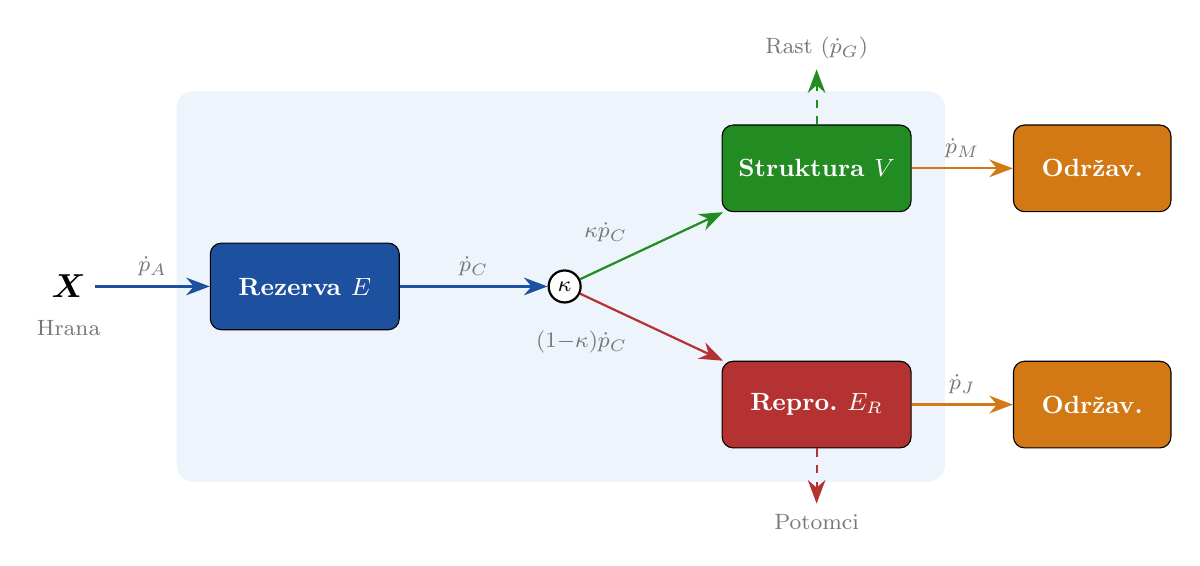
\begin{tikzpicture}[
    box/.style={rectangle, draw, rounded corners=4pt, minimum width=2.4cm,
                minimum height=1.1cm, font=\small\bfseries, text=white},
    flux/.style={-{Stealth[length=3mm]}, thick},
    label/.style={font=\footnotesize, text=debgrey},
  ]
  % Hrana
  \node[font=\large] (food) at (-4.5,0) {$\boldsymbol{X}$};
  \node[label, below=1pt of food] {Hrana};

  % Rezerva
  \node[box, fill=debblue] (E) at (-1.5,0) {Rezerva $E$};

  % Kappa split
  \node[circle, draw, thick, inner sep=2pt, fill=white,
        font=\footnotesize\bfseries] (kappa) at (1.8,0) {$\kappa$};

  % Struktura (soma)
  \node[box, fill=debgreen] (V) at (5,1.5) {Struktura $V$};

  % Reprodukcija
  \node[box, fill=debreduce] (R) at (5,-1.5) {Repro.\ $E_R$};

  % Odrzavanje soma
  \node[box, fill=deborange, minimum width=2cm] (Msom) at (8.5,1.5)
    {\small Odr\v{z}av.};

  % Odrzavanje zrelosti
  \node[box, fill=deborange, minimum width=2cm] (Mmat) at (8.5,-1.5)
    {\small Odr\v{z}av.};

  % Strelice
  \draw[flux, debblue] (food) -- node[above, label] {$\dot{p}_A$} (E);
  \draw[flux, debblue] (E) -- node[above, label] {$\dot{p}_C$} (kappa);

  \draw[flux, debgreen] (kappa) -- node[above left, label, pos=0.4]
    {$\kappa\dot{p}_C$} (V);
  \draw[flux, debreduce] (kappa) -- node[below left, label, pos=0.4]
    {$(1{-}\kappa)\dot{p}_C$} (R);

  \draw[flux, deborange] (V) -- node[above, label] {$\dot{p}_M$} (Msom);
  \draw[flux, deborange] (R) -- node[above, label] {$\dot{p}_J$} (Mmat);

  % Rast
  \draw[flux, debgreen, dashed] (V.north) -- ++(0,0.7)
    node[above, label] {Rast ($\dot{p}_G$)};

  % Potomci
  \draw[flux, debreduce, dashed] (R.south) -- ++(0,-0.7)
    node[below, label] {Potomci};

  % Pozadinski okvir
  \begin{scope}[on background layer]
    \node[fit=(E)(V)(R)(kappa), inner sep=12pt,
          fill=deblightblue, rounded corners=6pt, opacity=0.3] {};
  \end{scope}
\end{tikzpicture}
\caption{Shema tokova energije u standardnom DEB modelu ($\kappa$-pravilo).
  Energija iz hrane ulazi u rezervu $E$, mobilizira se i dijeli
  $\kappa$-pravilom: udio $\kappa$ ide na somatsko održavanje i rast
  strukture $V$, a ostatak $(1{-}\kappa)$ na održavanje zrelosti i
  reprodukciju $E_R$.}
\label{fig:deb-shema}
\end{figure}

Tokovi energije upravljaju se $\kappa$-pravilom: udio $\kappa$
mobilizirane rezerve odlazi na somatsko održavanje i rast, a ostatak na
održavanje zrelosti i reprodukciju.  Ključni tokovi su:
\begin{align}
  \dot{p}_A &= f\,\{p_{Am}\}\,L^2  &&\text{(asimilacija)}, \label{eq:pA}\\
  \dot{p}_C &= \frac{E\,v\,L}{E + [E_G]\,V}  &&\text{(mobilizacija)}, \label{eq:pC}\\
  \dot{p}_M &= [p_M]\,V  &&\text{(somatsko održavanje)}, \label{eq:pM}\\
  \frac{\mathrm{d}E}{\mathrm{d}t} &= \dot{p}_A - \dot{p}_C,  \label{eq:dE}\\
  \frac{\mathrm{d}V}{\mathrm{d}t} &= \frac{\kappa\,\dot{p}_C - \dot{p}_M}{[E_G]},  \label{eq:dV}\\
  \frac{\mathrm{d}E_R}{\mathrm{d}t} &= (1-\kappa)\,\dot{p}_C - \dot{p}_J.  \label{eq:dR}
\end{align}

Tablica~\ref{tab:params} prikazuje standardne DEB parametre korištene u
ovom paketu.

\begin{table}[htbp]
\centering
\caption{Standardni DEB parametri u paketu \pkg{BayesianDEB}.}
\label{tab:params}
\begin{tabular}{llll}
\toprule
\textbf{Simbol} & \textbf{R ime} & \textbf{Jedinice} & \textbf{Opis} \\
\midrule
$\{p_{Am}\}$ & \code{p\_Am} & J\,d$^{-1}$\,cm$^{-2}$ & Maks.\ specifična stopa asimilacije po površini \\
$[p_M]$      & \code{p\_M}  & J\,d$^{-1}$\,cm$^{-3}$ & Volumno-specifična stopa somatskog održavanja \\
$\kappa$     & \code{kappa} & -- & Udio alokacije na somu \\
$v$          & \code{v}     & cm\,d$^{-1}$ & Energetska vodljivost \\
$[E_G]$      & \code{E\_G}  & J\,cm$^{-3}$ & Specifični trošak strukture \\
$k_J$        & \code{k\_J}  & d$^{-1}$ & Stopa održavanja zrelosti \\
$E_H^p$      & \code{E\_Hp} & J & Zrelost pri pubertetu \\
$f$          & \code{f\_food} & -- & Skalirani funkcionalni odgovor (0--1) \\
$E_0$        & \code{E0}    & J\,cm$^{-3}$ & Početna gustoća rezervi \\
$L_0$        & \code{L0}    & cm & Početna strukturna duljina \\
$\sigma_L$   & \code{sigma\_L} & cm & Standardna devijacija pogreške opažanja \\
\bottomrule
\end{tabular}
\end{table}


% ============================================================
\section{Arhitektura paketa}
\label{sec:arhitektura}

\pkg{BayesianDEB} se sastoji od tri sloja:

\begin{description}[style=nextline]
  \item[Stan modeli] Unaprijed napisani \code{.stan} programi u direktoriju
    \code{inst/stan/} koji implementiraju DEB ODE sustav i Bayesovsku
    inferenciju.  Korisnici nikada ne trebaju izravno uređivati Stan kod.
  \item[R sučelje] Eksportirane funkcije za pripremu podataka,
    specifikaciju modela, procjenu, dijagnostiku i vizualizaciju.  Sve
    funkcije koriste S3 klase (\code{bdeb\_data}, \code{bdeb\_model},
    \code{bdeb\_fit}).
  \item[Sustav priora] Obitelj \code{prior\_*()} konstruktorskih funkcija
    koje kodiraju izbor distribucije kao lagane objekte proslijeđene
    funkciji \fn{bdeb\_model}.
\end{description}

\subsection{Ugrađeni Stan modeli}

\begin{table}[htbp]
\centering
\caption{Stan modeli ugrađeni u paket \pkg{BayesianDEB}.}
\label{tab:stan-modeli}
\begin{tabular}{lccl}
\toprule
\textbf{Stan datoteka} & \textbf{Stanja} & \textbf{R tip} & \textbf{Primjena} \\
\midrule
\code{bdeb\_individual\_growth} & $E, V$ & \code{"individual"} & Rast jednog organizma \\
\code{bdeb\_growth\_repro} & $E, V, R$ & \code{"growth\_repro"} & Rast + reprodukcija \\
\code{bdeb\_hierarchical\_growth} & $E, V$ + RE & \code{"hierarchical"} & Više jedinki, djelomično spajanje \\
\code{bdeb\_debtox} & $E, V, R, D_w$ & \code{"debtox"} & Ekotoksikologija (TKTD) \\
\bottomrule
\end{tabular}
\end{table}

Svi Stan modeli koriste BDF (eng.\ backward differentiation formula)
rješavač krutih ODE sustava (\code{ode\_bdf}) s tolerancijama $10^{-6}$
i maksimalno 10\,000 koraka, što je primjereno za razdvajanje vremenskih
skala tipično za DEB dinamiku rezervi i strukture.

\subsection{Radni tok}

Cjelokupni radni tok paketa može se sažeti sljedećim nizom poziva:

\begin{lstlisting}
bdeb_data() -> bdeb_model() -> bdeb_fit() -> bdeb_diagnose()
                                          -> bdeb_ppc()
                                          -> bdeb_derived()
                                          -> plot()
\end{lstlisting}

\begin{figure}[H]
\centering
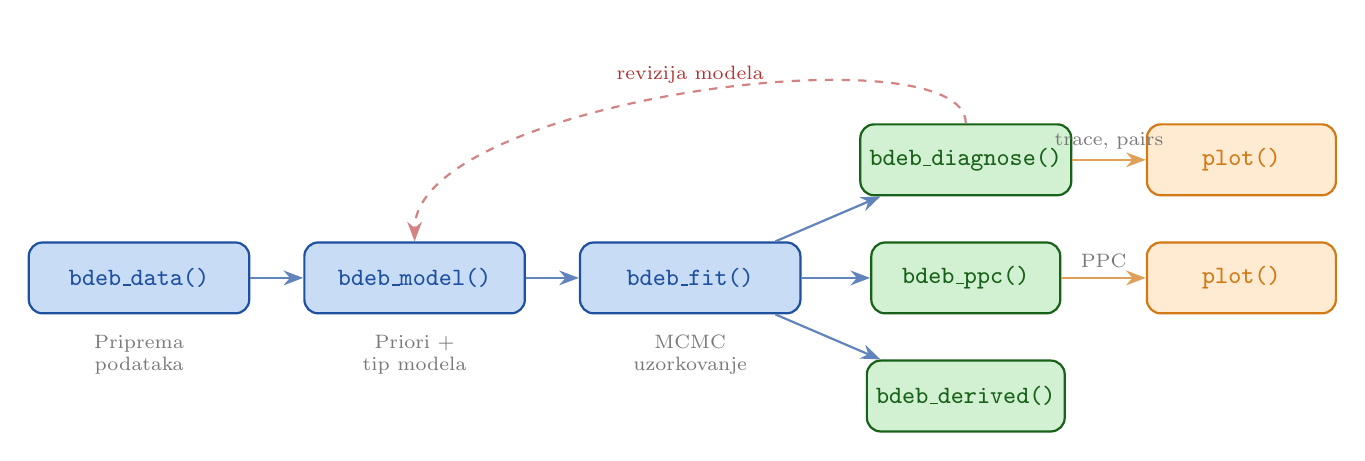
\begin{tikzpicture}[
    wfstep/.style={rectangle, draw=debblue, fill=deblightblue,
                 rounded corners=5pt, minimum width=2.8cm,
                 minimum height=0.9cm, font=\small\ttfamily,
                 text=debblue, thick, align=center},
    wfout/.style={rectangle, draw=debgreen!70!black, fill=deblightgreen,
                rounded corners=5pt, minimum width=2.4cm,
                minimum height=0.9cm, font=\small\ttfamily,
                text=debgreen!70!black, thick, align=center},
    arr/.style={-{Stealth[length=2.5mm]}, thick, debblue!70},
    note/.style={font=\scriptsize, text=debgrey, align=center},
  ]
  % Glavni tok
  \node[wfstep] (data) at (0,0) {bdeb\_data()};
  \node[wfstep] (model) at (3.5,0) {bdeb\_model()};
  \node[wfstep] (fit) at (7,0) {bdeb\_fit()};

  \draw[arr] (data) -- (model);
  \draw[arr] (model) -- (fit);

  % Grane iz fit
  \node[wfout] (diag) at (10.5,1.5) {bdeb\_diagnose()};
  \node[wfout] (ppc) at (10.5,0) {bdeb\_ppc()};
  \node[wfout] (derived) at (10.5,-1.5) {bdeb\_derived()};

  \draw[arr] (fit) -- (diag);
  \draw[arr] (fit) -- (ppc);
  \draw[arr] (fit) -- (derived);

  % Plot grane
  \node[wfout, fill=deblightorange, draw=deborange, text=deborange]
    (plot1) at (14,1.5) {plot()};
  \node[wfout, fill=deblightorange, draw=deborange, text=deborange]
    (plot2) at (14,0) {plot()};

  \draw[arr, deborange!70] (diag) -- node[above, note] {trace, pairs} (plot1);
  \draw[arr, deborange!70] (ppc) -- node[above, note] {PPC} (plot2);

  % Napomene ispod
  \node[note, below=4pt of data] {Priprema\\podataka};
  \node[note, below=4pt of model] {Priori +\\tip modela};
  \node[note, below=4pt of fit] {MCMC\\uzorkovanje};

  % Petlja revizije
  \draw[-{Stealth[length=2.5mm]}, thick, debreduce!60, dashed]
    (diag.north) .. controls +(0,1.2) and +(0,1.8) .. (model.north)
    node[midway, above, font=\scriptsize, text=debreduce] {revizija modela};
\end{tikzpicture}
\caption{Radni tok paketa \pkg{BayesianDEB}.  Isprekidana strelica
  označava iterativnu reviziju modela na temelju dijagnostike.}
\label{fig:radni-tok}
\end{figure}


% ============================================================
\section{Priprema podataka}
\label{sec:priprema}

\subsection{\fn{bdeb\_data} --- Priprema podataka za BDEB modele}

Funkcija \fn{bdeb\_data} pretvara podatkovne okvire u dugom formatu u
strukturirani format koji zahtijevaju Stan modeli.  Provodi validaciju
naziva stupaca, sortira po jedinkama i vremenu te konstruira interni S3
objekt klase \code{bdeb\_data}.

\begin{lstlisting}
bdeb_data(growth = NULL, reproduction = NULL,
          survival = NULL, concentration = NULL,
          f_food = 1.0)
\end{lstlisting}

\paragraph{Argumenti.}
\begin{description}[nosep,leftmargin=3.5cm,style=nextline]
  \item[\code{growth}] Podatkovni okvir sa stupcima \code{id}, \code{time},
    \code{length}.  Opcionalno i stupac \code{weight}.
  \item[\code{reproduction}] Podatkovni okvir sa stupcima \code{id},
    \code{t\_start}, \code{t\_end}, \code{count}.
  \item[\code{survival}] Podatkovni okvir sa stupcima \code{id},
    \code{time}, \code{event} (1~=~smrt, 0~=~cenzurirano).
  \item[\code{concentration}] Imenovani numerički vektor ili podatkovni
    okvir koji mapira ID-ove na vanjske koncentracije toksikanta (za
    DEBtox modele).
  \item[\code{f\_food}] Skalirani funkcionalni odgovor, $f \in [0,1]$.
    Zadano 1 (ad libitum hranjenje).
\end{description}

\paragraph{Vraća.} Objekt klase \code{bdeb\_data} (lista).

\paragraph{Primjer: jednostavni podaci o rastu.}
\begin{lstlisting}
library(BayesianDEB)

df <- data.frame(
  id     = rep(1, 10),
  time   = seq(0, 45, by = 5),
  length = c(0.10, 0.15, 0.22, 0.30, 0.38,
             0.44, 0.49, 0.52, 0.54, 0.55)
)
dat <- bdeb_data(growth = df)
dat
# -- BDEB Data ---
# i Individuals: 1
# i Endpoints: growth
# i Functional response (f): 1
# > Growth: 10 observations, t = [0, 45]
\end{lstlisting}

\paragraph{Primjer: korištenje ugrađenog dataseta.}
\begin{lstlisting}
data(eisenia_growth)
head(eisenia_growth)
#   id time length
# 1  1    0 0.1023
# 2  1    7 0.1487
# ...

# Jedna jedinka
dat1 <- bdeb_data(
  growth = eisenia_growth[eisenia_growth$id == 1, ],
  f_food = 1.0
)

# Sve jedinke (za hijerarhijski model)
dat_all <- bdeb_data(growth = eisenia_growth, f_food = 1.0)
dat_all
# => 21 jedinka, 273 opažanja
\end{lstlisting}

\paragraph{Primjer: kombinacija rasta i reprodukcije.}
\begin{lstlisting}
growth_df <- data.frame(
  id = 1, time = seq(0, 56, by = 7),
  length = c(0.10, 0.18, 0.28, 0.37, 0.44,
             0.49, 0.52, 0.54, 0.55)
)
repro_df <- data.frame(
  id      = 1,
  t_start = c(28, 35, 42, 49),
  t_end   = c(35, 42, 49, 56),
  count   = c(5, 12, 18, 15)
)
dat_gr <- bdeb_data(growth = growth_df,
                    reproduction = repro_df,
                    f_food = 1.0)
dat_gr
# => Endpoints: growth, reproduction
\end{lstlisting}

\paragraph{Primjer: podaci s koncentracijama (za DEBtox).}
\begin{lstlisting}
data(debtox_growth)

# Imenovanje koncentracijskih grupa
conc_map <- setNames(
  c(0, 20, 80, 200),
  as.character(unique(debtox_growth$concentration))
)

dat_tox <- bdeb_data(
  growth = debtox_growth,
  concentration = conc_map,
  f_food = 1.0
)
dat_tox
# => Concentration groups: 4
\end{lstlisting}


\subsection{\fn{repro\_to\_intervals} --- Pretvorba kumulativne reprodukcije u intervale}

Mnogi eksperimenti bilježe kumulativni broj potomaka.  Funkcija
\fn{repro\_to\_intervals} pretvara takve podatke u intervalne brojeve
prikladne za argument \code{reproduction} funkcije \fn{bdeb\_data}.

\begin{lstlisting}
repro_to_intervals(df)
\end{lstlisting}

\paragraph{Argumenti.}
\begin{description}[nosep,leftmargin=2.5cm]
  \item[\code{df}] Podatkovni okvir sa stupcima \code{id}, \code{time},
    \code{cumulative}.
\end{description}

\paragraph{Vraća.} Podatkovni okvir sa stupcima \code{id}, \code{t\_start},
\code{t\_end}, \code{count}.

\begin{lstlisting}
cumul <- data.frame(
  id         = rep(1, 5),
  time       = c(0, 7, 14, 21, 28),
  cumulative = c(0, 10, 30, 60, 100)
)
intervals <- repro_to_intervals(cumul)
intervals
#   id t_start t_end count
# 1  1       0     7    10
# 2  1       7    14    20
# 3  1      14    21    30
# 4  1      21    28    40
\end{lstlisting}


% ============================================================
\section{Specifikacija priora}
\label{sec:priori}

Priorne distribucije specificiraju se putem konstruktorskih funkcija koje
vraćaju objekte klase \code{bdeb\_prior}.  Ti se objekti predaju kao
imenovana lista funkciji \fn{bdeb\_model}; svi nespecificirani priori
automatski se popunjavaju iz funkcije \fn{prior\_default}.

\subsection{Konstruktori priora}

Paket nudi šest priornih distribucija prilagođenih različitim tipovima
DEB parametara:

\begin{longtable}{llll}
\toprule
\textbf{Funkcija} & \textbf{Distribucija} & \textbf{Argumenti} & \textbf{Preporučeno za} \\
\midrule
\endhead
\fn{prior\_lognormal} & $\text{LogNormal}(\mu, \sigma)$ & \code{mu, sigma} & Pozitivni parametri stope \\
\fn{prior\_normal} & $\mathcal{N}(\mu, \sigma)$ & \code{mu, sigma} & Neograničeni parametri \\
\fn{prior\_beta} & $\text{Beta}(a, b)$ & \code{a, b} & Parametri na $(0,1)$ \\
\fn{prior\_halfnormal} & $\text{HalfNormal}(\sigma)$ & \code{sigma} & Parametri skale \\
\fn{prior\_halfcauchy} & $\text{HalfCauchy}(\sigma)$ & \code{sigma} & Skala (teži repovi) \\
\fn{prior\_exponential} & $\text{Exp}(\lambda)$ & \code{rate} & Hijerarhijske varijance \\
\bottomrule
\end{longtable}

\paragraph{Preporuke za izbor priora.}
\begin{itemize}[nosep]
  \item \textbf{Pozitivni parametri stope} ($\{p_{Am}\}$, $[p_M]$, $v$,
    $[E_G]$, $k_J$, $k_d$, $z_w$, $b_w$): koristiti \fn{prior\_lognormal}.
  \item \textbf{Udio alokacije} ($\kappa$): koristiti \fn{prior\_beta}.
  \item \textbf{Standardna devijacija pogreške} ($\sigma_L$): koristiti
    \fn{prior\_halfnormal}.
  \item \textbf{Hijerarhijske komponente varijance}: koristiti
    \fn{prior\_exponential}.
\end{itemize}

\begin{figure}[H]
\centering
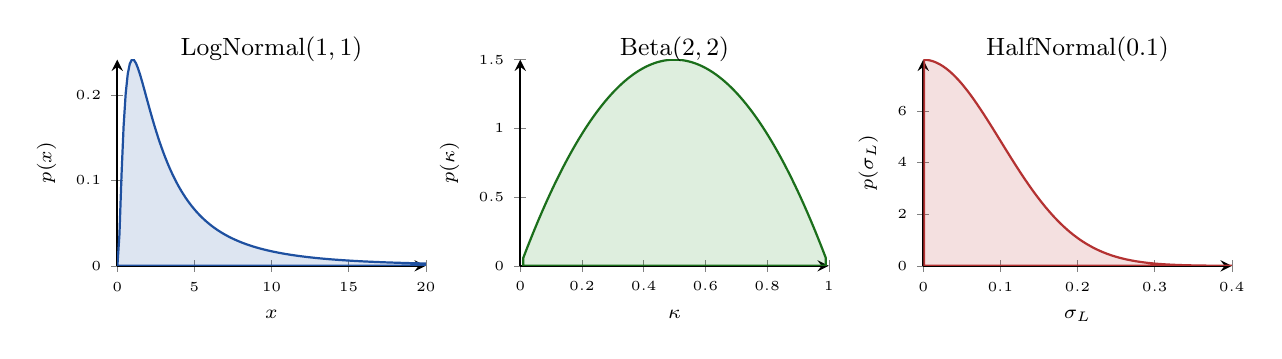
\begin{tikzpicture}
\begin{axis}[
    name=ax1, width=5.5cm, height=4.2cm,
    title={\small LogNormal$(1, 1)$},
    xlabel={$x$}, ylabel={$p(x)$},
    xmin=0, xmax=20, ymin=0,
    domain=0.01:20, samples=150,
    axis lines=left, thick,
    every axis title/.style={at={(0.5,1.05)}},
    xlabel style={font=\scriptsize},
    ylabel style={font=\scriptsize},
    tick label style={font=\tiny},
]
\addplot[thick, debblue, fill=debblue, fill opacity=0.15]
  {1/(x*1*sqrt(2*pi))*exp(-(ln(x)-1)^2/(2*1^2))} \closedcycle;
\end{axis}

\begin{axis}[
    at={(ax1.east)}, anchor=west, xshift=12mm,
    name=ax2, width=5.5cm, height=4.2cm,
    title={\small Beta$(2, 2)$},
    xlabel={$\kappa$}, ylabel={$p(\kappa)$},
    xmin=0, xmax=1, ymin=0,
    domain=0.01:0.99, samples=100,
    axis lines=left, thick,
    every axis title/.style={at={(0.5,1.05)}},
    xlabel style={font=\scriptsize},
    ylabel style={font=\scriptsize},
    tick label style={font=\tiny},
]
\addplot[thick, debgreen!80!black, fill=debgreen, fill opacity=0.15]
  {x^(2-1)*(1-x)^(2-1)*6} \closedcycle;
\end{axis}

\begin{axis}[
    at={(ax2.east)}, anchor=west, xshift=12mm,
    name=ax3, width=5.5cm, height=4.2cm,
    title={\small HalfNormal$(0.1)$},
    xlabel={$\sigma_L$}, ylabel={$p(\sigma_L)$},
    xmin=0, xmax=0.4, ymin=0,
    domain=0.001:0.4, samples=100,
    axis lines=left, thick,
    every axis title/.style={at={(0.5,1.05)}},
    xlabel style={font=\scriptsize},
    ylabel style={font=\scriptsize},
    tick label style={font=\tiny},
]
\addplot[thick, debreduce, fill=debreduce, fill opacity=0.15]
  {sqrt(2/(pi*0.1^2))*exp(-x^2/(2*0.1^2))} \closedcycle;
\end{axis}
\end{tikzpicture}
\caption{Oblici zadanih priornih distribucija korištenih u paketu:
  log-normalna za pozitivne parametre stope (lijevo),
  Beta za udio alokacije $\kappa$ (sredina),
  polu-normalna za parametre skale (desno).}
\label{fig:priori-oblici}
\end{figure}

\paragraph{Primjeri konstruktora.}
\begin{lstlisting}
# Log-normalni prior na stopu asimilacije
p1 <- prior_lognormal(mu = 1.5, sigma = 0.5)
p1$family  # "lognormal"
p1$mu      # 1.5

# Beta prior na kappu
p2 <- prior_beta(a = 3, b = 2)

# Polu-normalni prior na pogresku opazanja
p3 <- prior_halfnormal(sigma = 0.05)

# Eksponencijalni prior za hijerarhijsku varijancu
p4 <- prior_exponential(rate = 2)

# Normalni prior (za necentrirane parametre)
p5 <- prior_normal(mu = 1.5, sigma = 0.5)

# Polu-Cauchyjev prior (za robusnije repove)
p6 <- prior_halfcauchy(sigma = 1)
\end{lstlisting}


\subsection{\fn{prior\_default} --- Zadani slabo informativni priori}

Funkcija \fn{prior\_default} vraća kompletnu imenovanu listu slabo
informativnih priora prikladnih za zadani tip modela.

\begin{lstlisting}
prior_default(type = c("individual", "growth_repro",
                        "hierarchical", "debtox"))
\end{lstlisting}

Tablica~\ref{tab:zadani-priori} prikazuje zadane priore za individualni
model rasta.

\begin{table}[H]
\centering
\caption{Zadani priori za individualni model rasta.}
\label{tab:zadani-priori}
\begin{tabular}{lll}
\toprule
\textbf{Parametar} & \textbf{Prior} & \textbf{Obrazloženje} \\
\midrule
\code{p\_Am}    & $\text{LogNormal}(1.0,\; 1.0)$   & Pokriva raspon $\sim$0.4--20 \\
\code{p\_M}     & $\text{LogNormal}(-1.0,\; 1.0)$  & Pokriva raspon $\sim$0.04--2 \\
\code{kappa}    & $\text{Beta}(2,\; 2)$             & Favorizira unutarnje vrijednosti \\
\code{v}        & $\text{LogNormal}(-1.5,\; 1.0)$   & Pokriva raspon $\sim$0.02--1 \\
\code{E\_G}     & $\text{LogNormal}(6.0,\; 1.0)$    & Pokriva $\sim$100--3000 \\
\code{E0}       & $\text{LogNormal}(0.0,\; 1.0)$    & Početna gustoća rezervi \\
\code{L0}       & $\text{LogNormal}(-2.0,\; 1.0)$   & Početna duljina $\sim$0.01--0.5 \\
\code{sigma\_L} & $\text{HalfNormal}(0.1)$          & SD pogreške mjerenja \\
\bottomrule
\end{tabular}
\end{table}

Dodatni priori za specifične tipove modela:
\begin{itemize}[nosep]
  \item \code{"growth\_repro"} dodaje: \code{k\_J}, \code{E\_Hp},
    \code{k\_R} (pretvorba reproduktivnog spremnika u potomke),
    \code{phi\_R} (overdisperzija za negativnu binomnu).
  \item \code{"hierarchical"} dodaje: \code{mu\_log\_p\_Am}
    ($\mathcal{N}(1.0, 1.0)$), \code{sigma\_log\_p\_Am}
    ($\text{Exp}(1.0)$).
  \item \code{"debtox"} dodaje: \code{k\_d} (stopa oporavka štete),
    \code{z\_w} (NEC), \code{b\_w} (intenzitet učinka).
\end{itemize}

\begin{lstlisting}
# Pregled zadanih priora za svaki tip modela
prior_default("individual")
prior_default("growth_repro")
prior_default("hierarchical")
prior_default("debtox")
\end{lstlisting}


% ============================================================
\section{Modeli opažanja}
\label{sec:modeli-opazanja}

Modeli opažanja definiraju vezu između latentnih DEB stanja i mjerenih
podataka.  Specificiraju se putem konstruktorskih funkcija i predaju
argumentu \code{observation} funkcije \fn{bdeb\_model}.

\begin{longtable}{llll}
\toprule
\textbf{Funkcija} & \textbf{Distribucija} & \textbf{Zadano za} & \textbf{Primjena} \\
\midrule
\endhead
\fn{obs\_normal}    & $\mathcal{N}(\hat{L}, \sigma_L)$ & Rast & Kontinuirani podaci \\
\fn{obs\_lognormal} & $\text{LogNormal}(\log\hat{L}, \sigma)$ & -- & Multiplikativna pogreška \\
\fn{obs\_student\_t} & $t_\nu(\hat{L}, \sigma_L)$ & -- & Robusnost na stršeće vrijednosti \\
\fn{obs\_poisson}   & $\text{Poisson}(\Delta R)$ & -- & Brojčani podaci \\
\fn{obs\_negbinom}  & $\text{NegBin}(\Delta R, \phi)$ & Reprodukcija & Overdisperzirani brojevi \\
\bottomrule
\end{longtable}

\begin{lstlisting}
# Zadani modeli opazanja
obs_normal()           # za rast (Gaussovska pogreska)
obs_negbinom()         # za reprodukciju (negativna binomna)

# Alternativni izbori
obs_lognormal()        # multiplikativna pogreska
obs_student_t(nu = 5)  # robusno na strsece vrijednosti
obs_poisson()          # za rijetke dogadjaje
\end{lstlisting}


% ============================================================
\section{Specifikacija modela}
\label{sec:specifikacija}

\subsection{\fn{bdeb\_model} --- Specifikacija BDEB modela}

Funkcija \fn{bdeb\_model} kombinira podatke, tip DEB modela, priore i
model opažanja u jedinstvenu specifikaciju.  Ne provodi procjenu
modela---za to služi \fn{bdeb\_fit}.

\begin{lstlisting}
bdeb_model(data, type = c("individual", "growth_repro",
                           "hierarchical", "debtox"),
           priors = list(), observation = list(),
           temperature = NULL)
\end{lstlisting}

\paragraph{Argumenti.}
\begin{description}[nosep,leftmargin=3.5cm,style=nextline]
  \item[\code{data}] Objekt \code{bdeb\_data} kreiran s \fn{bdeb\_data}.
  \item[\code{type}] Tip modela (tablica~\ref{tab:stan-modeli}).
  \item[\code{priors}] Imenovana lista \code{bdeb\_prior} objekata.
    Nespecificirani priori popunjavaju se iz \fn{prior\_default}.
  \item[\code{observation}] Imenovana lista modela opažanja.  Zadano:
    \code{growth = obs\_normal()}, \code{reproduction = obs\_negbinom()}.
  \item[\code{temperature}] Opcionalna lista s komponentama \code{T}
    (temperatura opažanja u K), \code{T\_ref} (referentna temperatura),
    \code{T\_A} (Arrheniusova temperatura) za temperaturnu korekciju.
\end{description}

\paragraph{Vraća.} Objekt klase \code{bdeb\_model}.

\paragraph{Primjer: individualni model s prilagođenim priorima.}
\begin{lstlisting}
data(eisenia_growth)
df1 <- eisenia_growth[eisenia_growth$id == 1, ]
dat <- bdeb_data(growth = df1)

mod <- bdeb_model(dat, type = "individual",
  priors = list(
    p_Am    = prior_lognormal(mu = 1.5, sigma = 0.5),
    p_M     = prior_lognormal(mu = -1.0, sigma = 0.5),
    kappa   = prior_beta(a = 3, b = 2),
    sigma_L = prior_halfnormal(sigma = 0.05)
  ))
mod
# -- BDEB Model Specification ---
# i Type: individual
# i Stan model: bdeb_individual_growth
# i Individuals: 1
# -- Priors --
#   p_Am: LogNormal(1.5, 0.5)
#   kappa: Beta(3.0, 2.0)
#   ...
\end{lstlisting}

\paragraph{Primjer: hijerarhijski model sa zadanim priorima.}
\begin{lstlisting}
dat_all <- bdeb_data(growth = eisenia_growth)
mod_h <- bdeb_model(dat_all, type = "hierarchical")
# Svi priori automatski popunjeni iz prior_default("hierarchical")
mod_h
\end{lstlisting}

\paragraph{Primjer: model rasta i reprodukcije.}
\begin{lstlisting}
dat_gr <- bdeb_data(growth = growth_df,
                    reproduction = repro_df)
mod_gr <- bdeb_model(dat_gr, type = "growth_repro",
  priors = list(
    kappa = prior_beta(a = 3, b = 2),
    k_R   = prior_lognormal(mu = -2, sigma = 1)
  ))
\end{lstlisting}

\subsection{Validacija tipa i podataka}

Funkcija \fn{bdeb\_model} automatski provjerava kompatibilnost tipa
modela s dostupnim podacima:
\begin{itemize}[nosep]
  \item \code{"individual"}: upozorava ako postoji više od jedne jedinke
    (koristi samo prvu).
  \item \code{"growth\_repro"}: zahtijeva podatke o reprodukciji.
  \item \code{"debtox"}: zahtijeva podatke o koncentracijama.
\end{itemize}

\begin{lstlisting}
# Ovo ce javiti gresku jer nema podataka o reprodukciji:
# bdeb_model(dat, type = "growth_repro")

# Ovo ce javiti gresku jer nema podataka o koncentracijama:
# bdeb_model(dat, type = "debtox")
\end{lstlisting}


% ============================================================
\begin{figure}[H]
\centering
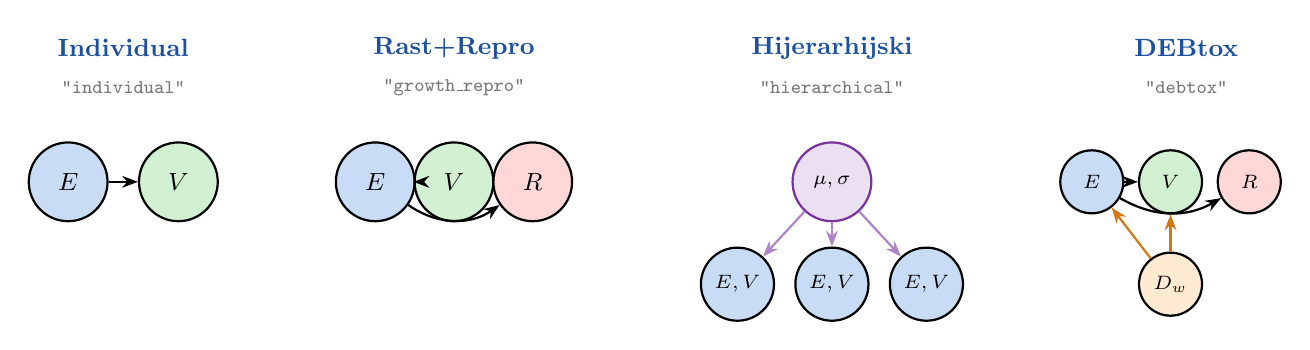
\begin{tikzpicture}[
    state/.style={circle, draw, thick, minimum size=1cm,
                  font=\small\bfseries},
    arr/.style={-{Stealth[length=2mm]}, thick},
    modlabel/.style={font=\small\bfseries, text=debblue},
    typelabel/.style={font=\scriptsize\ttfamily, text=debgrey},
  ]
  % --- Model 1: Individual (2-state) ---
  \node[modlabel] at (0, 2.2) {Individual};
  \node[typelabel] at (0, 1.7) {"individual"};
  \node[state, fill=deblightblue] (e1) at (-0.7, 0.5) {$E$};
  \node[state, fill=deblightgreen] (v1) at (0.7, 0.5) {$V$};
  \draw[arr] (e1) -- (v1);

  % --- Model 2: Growth+Repro (3-state) ---
  \node[modlabel] at (4.2, 2.2) {Rast+Repro};
  \node[typelabel] at (4.2, 1.7) {"growth\_repro"};
  \node[state, fill=deblightblue] (e2) at (3.2, 0.5) {$E$};
  \node[state, fill=deblightgreen] (v2) at (4.2, 0.5) {$V$};
  \node[state, fill=deblightred] (r2) at (5.2, 0.5) {$R$};
  \draw[arr] (e2) -- (v2);
  \draw[arr] (e2) to[bend right=35] (r2);

  % --- Model 3: Hierarchical (2-state + RE) ---
  \node[modlabel] at (9, 2.2) {Hijerarhijski};
  \node[typelabel] at (9, 1.7) {"hierarchical"};
  % Population level
  \node[state, fill=debpurple!15, draw=debpurple, font=\scriptsize\bfseries]
    (mu) at (9, 0.5) {$\mu,\sigma$};
  % Individual boxes
  \foreach \i/\xoff in {1/-1.2, 2/0, 3/1.2} {
    \node[state, fill=deblightblue, minimum size=0.7cm,
          font=\scriptsize\bfseries]
      (ind\i) at (9+\xoff, -0.8) {$E,V$};
    \draw[arr, debpurple!60] (mu) -- (ind\i);
  }

  % --- Model 4: DEBtox (4-state) ---
  \node[modlabel] at (13.5, 2.2) {DEBtox};
  \node[typelabel] at (13.5, 1.7) {"debtox"};
  \node[state, fill=deblightblue, minimum size=0.8cm,
        font=\scriptsize\bfseries] (e4) at (12.3, 0.5) {$E$};
  \node[state, fill=deblightgreen, minimum size=0.8cm,
        font=\scriptsize\bfseries] (v4) at (13.3, 0.5) {$V$};
  \node[state, fill=deblightred, minimum size=0.8cm,
        font=\scriptsize\bfseries] (r4) at (14.3, 0.5) {$R$};
  \node[state, fill=deblightorange, minimum size=0.8cm,
        font=\scriptsize\bfseries] (d4) at (13.3, -0.8) {$D_w$};
  \draw[arr] (e4) -- (v4);
  \draw[arr] (e4) to[bend right=30] (r4);
  \draw[arr, deborange] (d4) -- (e4);
  \draw[arr, deborange] (d4) -- (v4);
\end{tikzpicture}
\caption{Četiri tipa modela u paketu \pkg{BayesianDEB}.  $E$ = rezerva,
  $V$ = struktura, $R$ = reproduktivni spremnik, $D_w$ = skalirana
  unutarnja šteta, $\mu,\sigma$ = populacijski hiperparametri.}
\label{fig:tipovi-modela}
\end{figure}


\section{Procjena modela (MCMC)}
\label{sec:procjena}

\subsection{\fn{bdeb\_fit} --- Procjena BDEB modela}

Funkcija \fn{bdeb\_fit} kompilira Stan model (ako je potrebno) i pokreće
MCMC uzorkovanje putem \pkg{cmdstanr}-a.

\begin{lstlisting}
bdeb_fit(model, chains = 4, iter_warmup = 1000,
         iter_sampling = 1000, adapt_delta = 0.8,
         max_treedepth = 10, seed = NULL,
         parallel_chains = NULL, refresh = 200, ...)
\end{lstlisting}

\paragraph{Ključni argumenti.}
\begin{description}[nosep,leftmargin=3.5cm,style=nextline]
  \item[\code{model}] Objekt \code{bdeb\_model}.
  \item[\code{chains}] Broj MCMC lanaca.  Zadano 4.
  \item[\code{iter\_warmup}] Broj iteracija zagrijavanja po lancu.
    Zadano 1000.
  \item[\code{iter\_sampling}] Broj iteracija uzorkovanja po lancu.
    Zadano 1000.
  \item[\code{adapt\_delta}] Ciljna prosječna vjerojatnost prihvaćanja.
    Zadano 0.8.  Povećati prema 1.0 ako se pojave divergencije.
  \item[\code{max\_treedepth}] Maksimalna dubina stabla za NUTS.
    Zadano 10.
  \item[\code{seed}] Sjeme za reproduktivnost.
  \item[\code{parallel\_chains}] Broj lanaca koji se pokreću paralelno.
    Zadano: \code{min(chains, detectCores() - 1)}.
  \item[\code{refresh}] Učestalost ispisa napretka.  0 za tihi rad.
\end{description}

\paragraph{Vraća.} Objekt klase \code{bdeb\_fit} koji sadrži:
\begin{itemize}[nosep]
  \item \code{fit\$fit} --- sirovi \code{CmdStanMCMC} rezultat,
  \item \code{fit\$model} --- specifikacija modela,
  \item \code{fit\$stan\_model} --- kompilirani Stan model,
  \item metapodaci o uzorkovanju.
\end{itemize}

\paragraph{Primjer.}
\begin{lstlisting}
fit <- bdeb_fit(mod, chains = 4, iter_sampling = 2000,
                adapt_delta = 0.9, seed = 42)
fit
# -- BDEB Fit ---
# i Model type: individual
# i Chains: 4, Warmup: 1000, Sampling: 2000
# v No divergent transitions
\end{lstlisting}


% ============================================================
\section{Dijagnostika konvergencije}
\label{sec:dijagnostika}

\subsection{\fn{bdeb\_diagnose} --- MCMC dijagnostika}

Funkcija \fn{bdeb\_diagnose} ispisuje sveobuhvatno izvješće o
konvergenciji i automatski označava problematične vrijednosti.

\begin{lstlisting}
bdeb_diagnose(fit, pars = NULL)
\end{lstlisting}

Izvješće uključuje:
\begin{itemize}[nosep]
  \item \textbf{Divergentni prijelazi} --- prijelazi u kojima je NUTS
    sampler naišao na prijelom u geometriji posteriorne distribucije.  Idealno: 0.
  \item \textbf{Zasićenje dubine stabla} --- situacije u kojima je NUTS
    dosegao \code{max\_treedepth}.
  \item \textbf{E-BFMI} (energetski Bayesovski indeks frakcije nedostajuće
    informacije) --- vrijednosti $< 0.3$ ukazuju na neučinkovito
    uzorkovanje.
  \item \textbf{$\hat{R}$} --- mjera konvergencije lanaca.  Vrijednosti
    $> 1.01$ ukazuju na nedovoljnu konvergenciju.
  \item \textbf{ESS (bulk i tail)} --- efektivna veličina uzorka.
    Vrijednosti $< 400$ upozoravaju na nedovoljno uzorkovanje.
\end{itemize}

\begin{lstlisting}
diag <- bdeb_diagnose(fit)
# -- BDEB Diagnostics ---
# v No divergent transitions.
# v Treedepth OK.
# v E-BFMI OK (all > 0.3).
# -- Parameter Summary ---
# v All R-hat < 1.01.
# v Bulk ESS adequate (>400) for all parameters.
#   variable  mean    sd median    q5   q95  rhat ess_bulk ess_tail
#   p_Am      4.97  0.18   4.96  4.68  5.27  1.00     3240     2890
#   p_M       0.51  0.04   0.51  0.44  0.57  1.00     2780     2560
#   ...
\end{lstlisting}

\paragraph{Vraća (nevidljivo).} Lista s komponentama:
\code{n\_divergent}, \code{n\_max\_treedepth}, \code{ebfmi}, \code{summary}.


\subsection{\fn{bdeb\_summary} --- Posteriorna sumarizacija}

Funkcija \fn{bdeb\_summary} vraća urednu tablicu posteriornih
izvlačenja.

\begin{lstlisting}
bdeb_summary(fit, pars = NULL, prob = 0.90)
\end{lstlisting}

\paragraph{Argumenti.}
\begin{description}[nosep,leftmargin=2.5cm]
  \item[\code{pars}] Vektor imena parametara.  Zadano: svi parametri modela.
  \item[\code{prob}] Širina intervala vjerodostojnosti.  Zadano 0.90
    (5.\ i 95.\ percentil).
\end{description}

\begin{lstlisting}
# Svi parametri s 90% intervalom vjerodostojnosti
bdeb_summary(fit)

# Odabrani parametri s 95% intervalom
bdeb_summary(fit,
  pars = c("p_Am", "p_M", "kappa"),
  prob = 0.95)

# Funkcionira i preko S3 metode:
summary(fit)
\end{lstlisting}


% ============================================================
\section{Izvedene veličine}
\label{sec:izvedene}

\subsection{\fn{bdeb\_derived} --- Biološki značajne izvedene veličine}

Funkcija \fn{bdeb\_derived} izračunava izvedene veličine iz posteriornih
izvlačenja, automatski propagirajući nesigurnost.

\begin{lstlisting}
bdeb_derived(fit, quantities = c("L_inf", "k_M",
             "growth_rate"), f = 1.0)
\end{lstlisting}

Dostupne veličine:
\begin{itemize}[nosep]
  \item \code{"L\_inf"} --- konačna strukturna duljina:
    $L_\infty = f\,\kappa\,\{p_{Am}\} / [p_M]$.
  \item \code{"k\_M"} --- konstanta stope somatskog održavanja:
    $k_M = [p_M] / [E_G]$.
  \item \code{"growth\_rate"} --- von Bertalanffyjeva stopa rasta:
    $\dot{k} = \frac{v}{3}\,\frac{[p_M]}{\kappa\,[E_G]}$.
\end{itemize}

\paragraph{Vraća.} Objekt \code{posterior::draws\_df} s jednim stupcem po
traženoj veličini i jednim retkom po posteriornom izvlačenju.

\begin{lstlisting}
derived <- bdeb_derived(fit,
  quantities = c("L_inf", "growth_rate"))

# Sumarizacija izvedenih velicina
posterior::summarise_draws(derived,
  "mean", "sd",
  "q5"  = ~quantile(.x, 0.05),
  "q95" = ~quantile(.x, 0.95))
#   variable     mean     sd     q5    q95
#   L_inf        7.46   0.32   6.93   7.99
#   growth_rate  0.0033 0.0004 0.0027 0.0040

# Razliciti uvjeti hranjenja
bdeb_derived(fit,
  quantities = "L_inf", f = 0.7)  # smanjena hrana
\end{lstlisting}


% ============================================================
\section{Posteriorne prediktivne provjere (PPC)}
\label{sec:ppc}

\subsection{\fn{bdeb\_ppc} --- Provjera modela}

Posteriorne prediktivne provjere uspoređuju podatke generirane iz
posteriornog prediktivnog modela s opaženim podacima.  Stan modeli
generiraju replicirane podatke u bloku \code{generated quantities}.

\begin{lstlisting}
bdeb_ppc(fit, type = c("growth", "reproduction", "all"))
\end{lstlisting}

\paragraph{Vraća.} Objekt klase \code{bdeb\_ppc} koji sadrži:
\begin{itemize}[nosep]
  \item \code{growth\$L\_obs} --- opažene duljine,
  \item \code{growth\$L\_rep} --- matrica repliciranih duljina
    (redovi = izvlačenja, stupci = opažanja),
  \item \code{growth\$t\_obs} --- vremena opažanja.
\end{itemize}

\begin{lstlisting}
ppc <- bdeb_ppc(fit, type = "growth")
ppc
# -- BDEB Posterior Predictive Check ---
# i Type: growth
# > Growth: 13 observations, 4000 posterior draws

# Vizualizacija
plot(ppc, n_draws = 100)
\end{lstlisting}


\subsection{\fn{bdeb\_predict} i \fn{predict.bdeb\_fit} --- Predikcije}

Generira posteriorne prediktivne trajektorije.

\begin{lstlisting}
bdeb_predict(fit, newdata = NULL, n_draws = 200)
# ili ekvivalentno:
predict(fit, n_draws = 200)
\end{lstlisting}

\begin{lstlisting}
pred <- predict(fit, n_draws = 100)
# pred$t      - vremenski niz
# pred$L_hat  - matrica predvidenih duljina
# pred$n_draws - broj izvlacenja
\end{lstlisting}


% ============================================================
\section{Vizualizacija}
\label{sec:vizualizacija}

\pkg{BayesianDEB} nudi raznolike grafičke prikaze za dijagnostiku,
interpretaciju i publikaciju.  Svi grafovi vraćaju objekte paketa
\pkg{ggplot2} koji se mogu dalje prilagođavati.

\subsection{\code{plot(fit, type = ...)} --- Grafički prikazi procjene}

\begin{lstlisting}
plot(fit, type = c("trace", "posterior", "pairs",
                    "trajectory"),
     pars = NULL, n_draws = 100)
\end{lstlisting}

\subsubsection{Trace grafovi}

Prikazuju MCMC lance kroz iteracije za vizualnu procjenu konvergencije.
Lanci koji se dobro miješaju trebaju izgledati kao ``dlakavi crvi'' koji
se preklapaju.

\begin{lstlisting}
plot(fit, type = "trace")

# Odabrani parametri
plot(fit, type = "trace",
     pars = c("p_Am", "kappa", "sigma_L"))
\end{lstlisting}

\begin{figure}[H]
\centering
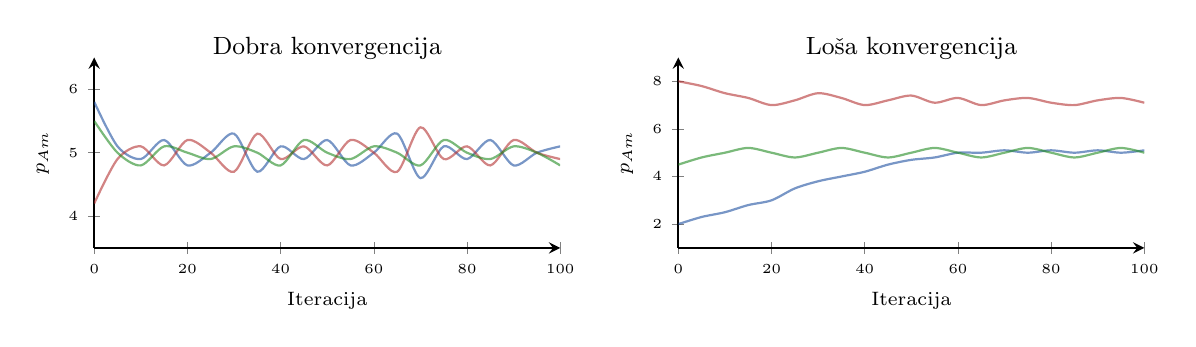
\begin{tikzpicture}
% --- Dobar trace (konvergirani lanci) ---
\begin{axis}[
    name=good, width=7.5cm, height=4cm,
    title={\small Dobra konvergencija},
    xlabel={\scriptsize Iteracija}, ylabel={\scriptsize $p_{Am}$},
    xmin=0, xmax=100, ymin=3.5, ymax=6.5,
    axis lines=left, thick,
    tick label style={font=\tiny},
    xlabel style={font=\scriptsize},
    ylabel style={font=\scriptsize},
    every axis title/.style={at={(0.5,1.05)}},
]
% Lanac 1 (plavi)
\addplot[debblue, opacity=0.6, thick, smooth]
  coordinates {
    (0,5.8)(5,5.1)(10,4.9)(15,5.2)(20,4.8)(25,5.0)(30,5.3)(35,4.7)
    (40,5.1)(45,4.9)(50,5.2)(55,4.8)(60,5.0)(65,5.3)(70,4.6)(75,5.1)
    (80,4.9)(85,5.2)(90,4.8)(95,5.0)(100,5.1)
  };
% Lanac 2 (crveni)
\addplot[debreduce, opacity=0.6, thick, smooth]
  coordinates {
    (0,4.2)(5,4.9)(10,5.1)(15,4.8)(20,5.2)(25,5.0)(30,4.7)(35,5.3)
    (40,4.9)(45,5.1)(50,4.8)(55,5.2)(60,5.0)(65,4.7)(70,5.4)(75,4.9)
    (80,5.1)(85,4.8)(90,5.2)(95,5.0)(100,4.9)
  };
% Lanac 3 (zeleni)
\addplot[debgreen, opacity=0.6, thick, smooth]
  coordinates {
    (0,5.5)(5,5.0)(10,4.8)(15,5.1)(20,5.0)(25,4.9)(30,5.1)(35,5.0)
    (40,4.8)(45,5.2)(50,5.0)(55,4.9)(60,5.1)(65,5.0)(70,4.8)(75,5.2)
    (80,5.0)(85,4.9)(90,5.1)(95,5.0)(100,4.8)
  };
\end{axis}

% --- Los trace (nekonvergirani lanci) ---
\begin{axis}[
    at={(good.east)}, anchor=west, xshift=15mm,
    width=7.5cm, height=4cm,
    title={\small Lo\v{s}a konvergencija},
    xlabel={\scriptsize Iteracija}, ylabel={\scriptsize $p_{Am}$},
    xmin=0, xmax=100, ymin=1, ymax=9,
    axis lines=left, thick,
    tick label style={font=\tiny},
    xlabel style={font=\scriptsize},
    ylabel style={font=\scriptsize},
    every axis title/.style={at={(0.5,1.05)}},
]
\addplot[debblue, opacity=0.6, thick, smooth]
  coordinates {
    (0,2)(5,2.3)(10,2.5)(15,2.8)(20,3.0)(25,3.5)(30,3.8)(35,4.0)
    (40,4.2)(45,4.5)(50,4.7)(55,4.8)(60,5.0)(65,5.0)(70,5.1)(75,5.0)
    (80,5.1)(85,5.0)(90,5.1)(95,5.0)(100,5.1)
  };
\addplot[debreduce, opacity=0.6, thick, smooth]
  coordinates {
    (0,8)(5,7.8)(10,7.5)(15,7.3)(20,7.0)(25,7.2)(30,7.5)(35,7.3)
    (40,7.0)(45,7.2)(50,7.4)(55,7.1)(60,7.3)(65,7.0)(70,7.2)(75,7.3)
    (80,7.1)(85,7.0)(90,7.2)(95,7.3)(100,7.1)
  };
\addplot[debgreen, opacity=0.6, thick, smooth]
  coordinates {
    (0,4.5)(5,4.8)(10,5.0)(15,5.2)(20,5.0)(25,4.8)(30,5.0)(35,5.2)
    (40,5.0)(45,4.8)(50,5.0)(55,5.2)(60,5.0)(65,4.8)(70,5.0)(75,5.2)
    (80,5.0)(85,4.8)(90,5.0)(95,5.2)(100,5.0)
  };
\end{axis}
\end{tikzpicture}
\caption{Primjeri trace grafova.  Lijevo: tri lanca se dobro miješaju
  (konvergencija).  Desno: lanci se ne preklapaju (nedovoljna
  konvergencija, $\hat{R} > 1.01$).}
\label{fig:trace-primjeri}
\end{figure}

\subsubsection{Posteriorne gustoće}

Preklopljene marginalne posteriorne distribucije po lancima.

\begin{lstlisting}
plot(fit, type = "posterior")
plot(fit, type = "posterior",
     pars = c("p_Am", "p_M", "kappa"))
\end{lstlisting}

\subsubsection{Dijagrami parova}

Bivarijatni dijagrami rasipanja koji prikazuju posteriorne korelacije
između parametara.  Korisni za otkrivanje degeneracija i jakih korelacija.

\begin{lstlisting}
plot(fit, type = "pairs",
     pars = c("p_Am", "p_M", "kappa"))
\end{lstlisting}

\subsubsection{Trajektorije}

Posteriorno predviđene krivulje rasta preklopljene s opaženim podacima.

\begin{lstlisting}
plot(fit, type = "trajectory", n_draws = 200)
# Plave linije = posteriorna predvidanja
# Crne tocke = opazeni podaci
\end{lstlisting}

\subsection{\code{plot(ppc)} --- Grafički prikaz PPC-a}

\begin{lstlisting}
ppc <- bdeb_ppc(fit, type = "growth")
plot(ppc, n_draws = 50)
# Sive linije = replicirane trajektorije
# Crvene tocke = opazeni podaci
\end{lstlisting}

Za reprodukciju, PPC grafikon prikazuje histogram repliciranih brojeva
potomaka s okomitim linijama za opažene vrijednosti.


% ============================================================
\section{DEBtox: Ekotoksikološki modeli}
\label{sec:debtox}

DEBtox modeli kombiniraju DEB energetiku s toksikokinetičko-toksikodinamičkim
(TKTD) okvirom za procjenu učinaka kemikalija na organizme.

\begin{figure}[H]
\centering
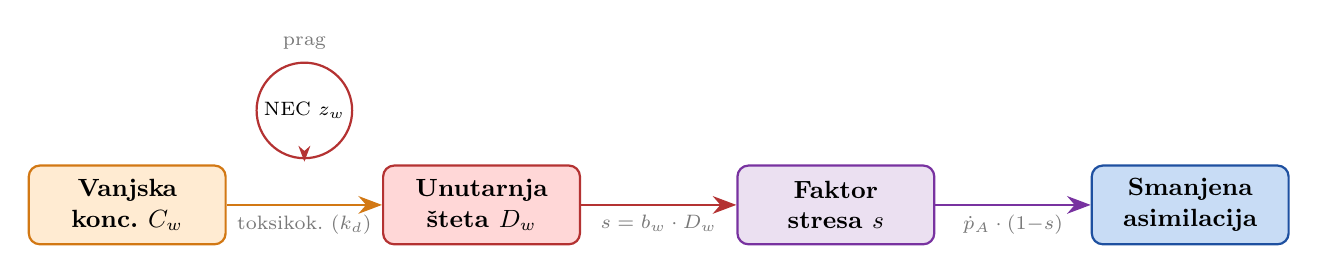
\begin{tikzpicture}[
    box/.style={rectangle, draw, rounded corners=4pt, thick,
                minimum width=2.5cm, minimum height=1cm,
                font=\small\bfseries, align=center},
    arr/.style={-{Stealth[length=3mm]}, thick},
    note/.style={font=\scriptsize, text=debgrey},
  ]
  % Vanjska koncentracija
  \node[box, fill=deblightorange, draw=deborange] (Cw) at (0,0)
    {Vanjska\\konc.\ $C_w$};

  % Unutarnja steta
  \node[box, fill=deblightred, draw=debreduce] (Dw) at (4.5,0)
    {Unutarnja\\\v{s}teta $D_w$};

  % Stres faktor
  \node[box, fill=debpurple!15, draw=debpurple] (stress) at (9,0)
    {Faktor\\stresa $s$};

  % Efekt na DEB
  \node[box, fill=deblightblue, draw=debblue] (effect) at (13.5,0)
    {Smanjena\\asimilacija};

  % NEC prag
  \node[circle, draw=debreduce, thick, inner sep=2pt, fill=white,
        font=\scriptsize] (nec) at (2.25,1.2) {NEC $z_w$};

  % Strelice
  \draw[arr, deborange] (Cw) -- node[below, note]
    {toksikok.\ ($k_d$)} (Dw);
  \draw[arr, debreduce] (Dw) -- node[below, note]
    {$s = b_w \cdot D_w$} (stress);
  \draw[arr, debpurple] (stress) -- node[below, note]
    {$\dot{p}_A \cdot (1{-}s)$} (effect);

  % NEC prag strelica
  \draw[-{Stealth[length=2mm]}, thick, debreduce, dashed]
    (nec) -- (2.25,0.55);
  \node[note, above=1pt of nec] {prag};
\end{tikzpicture}
\caption{Shema TKTD okvira u DEBtox modelu.  Vanjska koncentracija
  ulazi u organizam i uzrokuje unutarnju štetu $D_w$ iznad praga NEC
  ($z_w$).  Šteta se prevodi u faktor stresa $s$ koji smanjuje
  asimilaciju.}
\label{fig:tktd-shema}
\end{figure}

\subsection{Teorijska pozadina}

Model dodaje varijablu skalirane unutarnje štete $D_w$ čija dinamika
slijedi:
\begin{equation}
\frac{\mathrm{d}D_w}{\mathrm{d}t} = k_d\bigl(\max(C_w - z_w,\, 0) - D_w\bigr),
\end{equation}
gdje je $k_d$ stopa oporavka od štete, $z_w$ je koncentracija bez učinka
(NEC --- No Effect Concentration), a $C_w$ je vanjska koncentracija.

Faktor stresa koji djeluje na asimilaciju:
\begin{equation}
s = b_w \cdot \max(D_w,\, 0), \qquad
\dot{p}_A = f\,\{p_{Am}\}\,L^2 \cdot \max(1 - s,\, 0).
\end{equation}

U stacionarnom stanju $D_w = \max(C_w - z_w, 0)$, pa se $\text{EC}_{50}$
izračunava analitički:
\begin{equation}
\text{EC}_{50} = z_w + \frac{0.5}{b_w}.
\end{equation}

\subsection{Dodatni DEBtox parametri}

\begin{table}[H]
\centering
\caption{Parametri specifični za DEBtox model.}
\begin{tabular}{llll}
\toprule
\textbf{Simbol} & \textbf{R ime} & \textbf{Jedinice} & \textbf{Opis} \\
\midrule
$k_d$ & \code{k\_d} & d$^{-1}$ & Stopa oporavka od štete \\
$z_w$ & \code{z\_w} & konc.\ jedinice & NEC (koncentracija bez učinka) \\
$b_w$ & \code{b\_w} & 1/konc.\ jedinice & Intenzitet učinka \\
\bottomrule
\end{tabular}
\end{table}

\subsection{\fn{bdeb\_tox} --- Specifikacija DEBtox modela}

Pogodnosna ovojnica oko \fn{bdeb\_model} s \code{type = "debtox"}.

\begin{lstlisting}
bdeb_tox(data, stress = c("assimilation", "maintenance",
         "growth_cost"), priors = list(), ...)
\end{lstlisting}

Trenutačno je implementiran samo stres na asimilaciju.  Buduće verzije
uključit će stres na održavanje i trošak rasta.

\begin{lstlisting}
data(debtox_growth)

conc_map <- setNames(
  c(0, 20, 80, 200),
  as.character(unique(debtox_growth$concentration))
)

dat_tox <- bdeb_data(
  growth = debtox_growth,
  concentration = conc_map
)

mod_tox <- bdeb_tox(dat_tox, stress = "assimilation",
  priors = list(
    z_w = prior_lognormal(mu = 2.5, sigma = 1.0),
    b_w = prior_lognormal(mu = -5.0, sigma = 2.0)
  ))

fit_tox <- bdeb_fit(mod_tox, chains = 4,
                    adapt_delta = 0.95, seed = 77)
\end{lstlisting}


\begin{figure}[H]
\centering
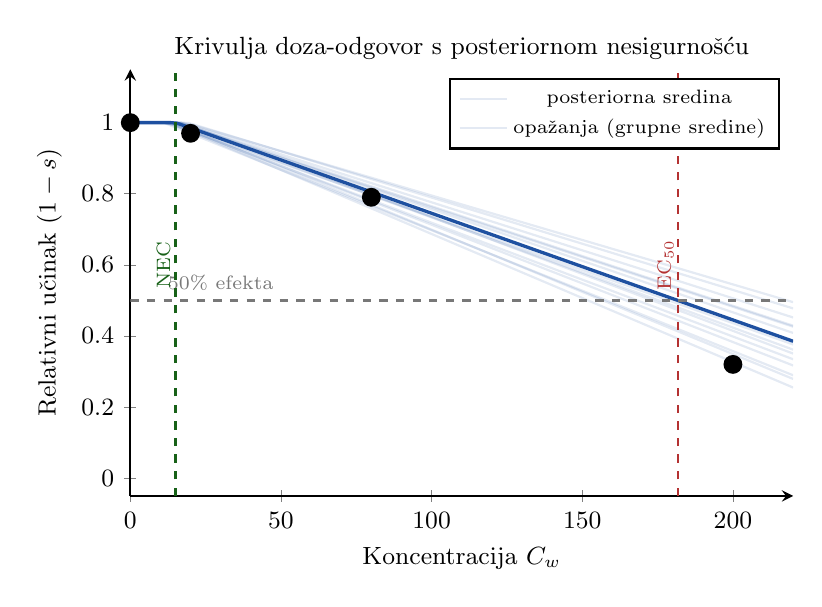
\begin{tikzpicture}
\begin{axis}[
    width=10cm, height=7cm,
    title={\small Krivulja doza-odgovor s posteriornom nesigurno\v{s}\'{c}u},
    xlabel={Koncentracija $C_w$},
    ylabel={Relativni u\v{c}inak $(1 - s)$},
    xmin=0, xmax=220, ymin=-0.05, ymax=1.15,
    axis lines=left, thick,
    tick label style={font=\small},
    xlabel style={font=\small},
    ylabel style={font=\small},
    every axis title/.style={at={(0.5,1.05)}, font=\small},
    legend style={font=\scriptsize, at={(0.98,0.98)}, anchor=north east},
]
% Posteriorne linije (prozirne plave)
\foreach \nec/\bw in {
  12/0.0032, 16/0.0028, 14/0.0035, 18/0.0025, 13/0.0033,
  15/0.0030, 17/0.0027, 11/0.0034, 19/0.0026, 14/0.0031,
  16/0.0029, 13/0.0036, 15/0.0028, 17/0.0032, 12/0.0030} {
  \addplot[debblue, opacity=0.12, thick, domain=0:220, samples=80]
    {max(1 - \bw * max(x - \nec, 0), 0)};
}
% Srednja krivulja
\addplot[debblue, very thick, domain=0:220, samples=100]
  {max(1 - 0.003 * max(x - 15, 0), 0)};
\addlegendentry{posteriorna sredina}

% EC50 linija
\addplot[dashed, thick, debgrey] coordinates {(0,0.5) (220,0.5)};
\node[font=\scriptsize, debgrey] at (30, 0.55) {50\% efekta};

% NEC
\addplot[dashed, thick, debgreen!70!black]
  coordinates {(15,-0.05) (15,1.15)};
\node[font=\scriptsize, debgreen!70!black, rotate=90] at (11, 0.6) {NEC};

% EC50
\pgfmathsetmacro{\ecval}{15 + 0.5/0.003}
\addplot[dashed, thick, debreduce]
  coordinates {(\ecval,-0.05) (\ecval,1.15)};
\node[font=\scriptsize, debreduce, rotate=90] at (\ecval-4, 0.6) {EC$_{50}$};

% Opazene tocke (grupirane srednje)
\addplot[only marks, mark=*, mark size=3pt, black]
  coordinates {(0,1.0) (20,0.97) (80,0.79) (200,0.32)};
\addlegendentry{opa\v{z}anja (grupne sredine)}
\end{axis}
\end{tikzpicture}
\caption{Krivulja doza-odgovor generirana funkcijom
  \fn{plot\_dose\_response}.  Plave prozirne linije prikazuju
  posteriorne izvlačenja funkcije stresa.  Vertikalne isprekidane
  linije označavaju NEC (zeleno) i EC$_{50}$ (crveno).}
\label{fig:doza-odgovor}
\end{figure}


\subsection{\fn{bdeb\_ec50} --- Ekstrakcija EC50 i NEC}

Ekstrahira posteriornu distribuciju $\text{EC}_{50}$ i NEC iz procijenjenog
DEBtox modela.

\begin{lstlisting}
bdeb_ec50(fit, prob = 0.90)
\end{lstlisting}

\paragraph{Vraća.} Lista s komponentama:
\begin{itemize}[nosep]
  \item \code{draws} --- posteriorna izvlačenja EC50,
  \item \code{summary} --- podatkovni okvir s mean, median, sd, lower, upper,
  \item \code{NEC} --- sumarizacija koncentracije bez učinka.
\end{itemize}

\begin{lstlisting}
result <- bdeb_ec50(fit_tox, prob = 0.95)
# -- DEBtox Effect Concentrations ---
#   parameter  mean median    sd lower upper
#       EC50  181.7  180.2  12.4 159.3 204.1
#        NEC   15.3   15.1   2.1  11.8  19.2

# Pristup posteriornim izvlacenjima
hist(result$draws, breaks = 40,
     main = "Posteriorna distribucija EC50",
     xlab = "Koncentracija")
\end{lstlisting}


\subsection{\fn{plot\_dose\_response} --- Krivulja doza-odgovor}

Prikazuje funkciju stresa preko kontinuiranog raspona koncentracija s
pojasima posteriorne nesigurnosti.

\begin{lstlisting}
plot_dose_response(fit, endpoint = "growth",
                   n_draws = 100)
\end{lstlisting}

\begin{lstlisting}
plot_dose_response(fit_tox, n_draws = 200)
# Plave linije = posteriorna predvidanja stresa
# Crvene tocke = opazene relativne vrijednosti
# Isprekidana linija = 50% efekta (za EC50)
\end{lstlisting}


% ============================================================
\section{Pomoćne funkcije}
\label{sec:pomocne}

\subsection{\fn{arrhenius} --- Arrheniusova temperaturna korekcija}

Izračunava korekcijski faktor za DEB parametre stope na temelju
Arrheniusovog odnosa:
\begin{equation}
c_T = \exp\!\left(\frac{T_A}{T_{\text{ref}}} - \frac{T_A}{T}\right).
\end{equation}

\begin{figure}[H]
\centering
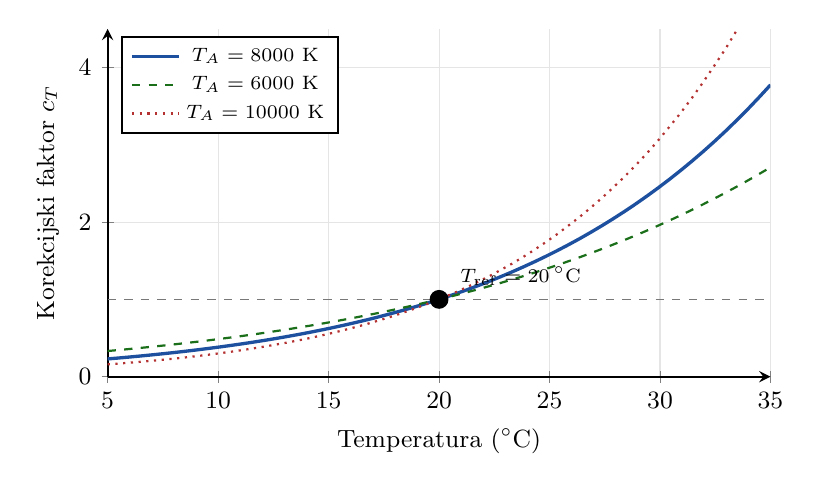
\begin{tikzpicture}
\begin{axis}[
    width=10cm, height=6cm,
    xlabel={Temperatura ($^\circ$C)},
    ylabel={Korekcijski faktor $c_T$},
    xmin=5, xmax=35, ymin=0, ymax=4.5,
    axis lines=left, thick,
    tick label style={font=\small},
    xlabel style={font=\small},
    ylabel style={font=\small},
    legend style={font=\scriptsize, at={(0.02,0.98)}, anchor=north west},
    grid=major, grid style={gray!20},
]
% T_A = 8000 (standardni)
\addplot[debblue, very thick, domain=5:35, samples=60]
  {exp(8000/293.15 - 8000/(x+273.15))};
\addlegendentry{$T_A = 8000$ K}

% T_A = 6000
\addplot[debgreen!80!black, thick, dashed, domain=5:35, samples=60]
  {exp(6000/293.15 - 6000/(x+273.15))};
\addlegendentry{$T_A = 6000$ K}

% T_A = 10000
\addplot[debreduce, thick, dotted, domain=5:35, samples=60]
  {exp(10000/293.15 - 10000/(x+273.15))};
\addlegendentry{$T_A = 10000$ K}

% Referentna tocka
\addplot[only marks, mark=*, mark size=3pt, black]
  coordinates {(20,1.0)};
\node[font=\scriptsize, anchor=south west] at (20.5,1.05)
  {$T_\mathrm{ref}=20\,^\circ$C};

% Horizontalna linija na c_T = 1
\addplot[debgrey, thin, dashed] coordinates {(5,1) (35,1)};
\end{axis}
\end{tikzpicture}
\caption{Arrheniusov korekcijski faktor $c_T$ u ovisnosti o temperaturi
  za tri vrijednosti Arrheniusove temperature $T_A$.  Pri referentnoj
  temperaturi ($20\,^\circ$C) faktor je uvijek 1.}
\label{fig:arrhenius}
\end{figure}

\begin{lstlisting}
arrhenius(T, T_ref = 293.15, T_A = 8000)
\end{lstlisting}

\begin{lstlisting}
# Pri referentnoj temperaturi (20 C): faktor = 1
arrhenius(293.15)
# [1] 1

# Pri 25 C (5 stupnjeva toplije): faktor > 1
arrhenius(298.15)
# [1] 1.741

# Pri 15 C (5 stupnjeva hladnije): faktor < 1
arrhenius(288.15)
# [1] 0.552

# Prilagodeni Arrheniusov parametar
arrhenius(298.15, T_ref = 293.15, T_A = 6000)
\end{lstlisting}


\subsection{\fn{deb\_fluxes} --- Izračun DEB energetskih tokova}

Za zadano trenutačno stanje $(E, V)$ i parametre izračunava sve
standardne DEB energetske tokove.

\begin{lstlisting}
deb_fluxes(E, V, f, p_Am, p_M, kappa, v, E_G,
           k_J = 0, E_Hp = 0)
\end{lstlisting}

\paragraph{Vraća.} Imenovana lista s tokovima: \code{p\_A} (asimilacija),
\code{p\_C} (mobilizacija), \code{p\_M} (somatsko održavanje),
\code{p\_G} (rast), \code{p\_J} (održavanje zrelosti), \code{p\_R}
(reprodukcija), te izvedene veličine \code{L} (strukturna duljina) i
\code{e} (skalirana gustoća rezervi).

\begin{lstlisting}
fl <- deb_fluxes(E = 10, V = 0.5, f = 1.0,
                 p_Am = 5, p_M = 0.5, kappa = 0.75,
                 v = 0.2, E_G = 400)

fl$p_A  # tok asimilacije
fl$p_C  # tok mobilizacije
fl$p_M  # tok somatskog odrzavanja
fl$p_G  # tok rasta
fl$L    # strukturna duljina = V^(1/3)
fl$e    # skalirana gustoca rezervi

# Primjer za organizam s reprodukcijom
fl2 <- deb_fluxes(E = 50, V = 2.0, f = 1.0,
                  p_Am = 5, p_M = 0.5, kappa = 0.75,
                  v = 0.2, E_G = 400,
                  k_J = 0.002, E_Hp = 50)
fl2$p_R  # tok reprodukcije
fl2$p_J  # tok odrzavanja zrelosti
\end{lstlisting}


% ============================================================
\section{Ugrađeni skupovi podataka}
\label{sec:dataseti}

Paket uključuje tri simulirana skupa podataka za demonstraciju i testiranje.

\subsection{\code{eisenia\_growth}}

Simulirani podaci o rastu za 21 jedinku gliste \textit{Eisenia fetida}
mjerenu tjedno kroz 12 tjedana (dani 0, 7, 14, \ldots, 84).

\begin{description}[nosep,leftmargin=3cm]
  \item[Redaka] 273 (21 jedinka $\times$ 13 vremenskih točaka).
  \item[Stupci] \code{id} (cijeli broj 1--21), \code{time} (dani), \code{length} (cm).
  \item[Stvarni parametri] $\{p_{Am}\} = 5.0$, $[p_M] = 0.5$, $\kappa = 0.75$,
    $v = 0.2$, $[E_G] = 400$; individualna varijacija u $\{p_{Am}\}$
    (CV $\approx$ 10\%) i $L_0$ (CV $\approx$ 5\%); $\sigma_L = 0.015$\,cm.
\end{description}

\begin{lstlisting}
data(eisenia_growth)
head(eisenia_growth)
str(eisenia_growth)

# Vizualizacija
library(ggplot2)
ggplot(eisenia_growth, aes(time, length, group = id)) +
  geom_line(alpha = 0.4) +
  theme_bw() +
  labs(x = "Vrijeme (dani)", y = "Strukturna duljina (cm)")
\end{lstlisting}

\begin{figure}[H]
\centering
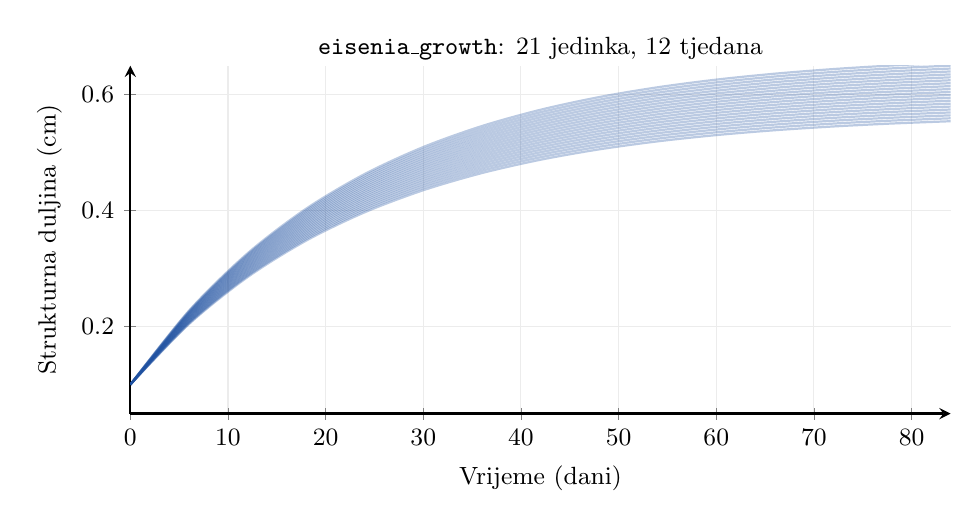
\begin{tikzpicture}
\begin{axis}[
    width=12cm, height=6cm,
    xlabel={Vrijeme (dani)},
    ylabel={Strukturna duljina (cm)},
    xmin=0, xmax=84, ymin=0.05, ymax=0.65,
    axis lines=left, thick,
    tick label style={font=\small},
    xlabel style={font=\small},
    ylabel style={font=\small},
    grid=major, grid style={gray!15},
    title={\small \code{eisenia\_growth}: 21 jedinka, 12 tjedana},
    every axis title/.style={at={(0.5,1.05)}, font=\small},
]
% Simulirane trajektorije za 8 jedinki s varijacijom u p_Am
% 21 trajektorija s varijacijom u p_Am
\foreach \s in {1.00,1.05,0.95,1.08,0.92,1.03,0.97,1.10,0.90,1.02,
                0.98,1.06,0.94,1.04,0.96,1.07,0.93,1.01,0.99,1.09,0.91} {
  \addplot[debblue, opacity=0.3, thick, smooth, domain=0:84, samples=15]
    {\s * 0.52 * (1 - exp(-0.042*x)) + 0.10};
}
\end{axis}
\end{tikzpicture}
\caption{Ilustracija podataka \code{eisenia\_growth}: krivulje rasta
  za 21 jedinku gliste \textit{Eisenia fetida} s individualnom
  varijacijom u stopi asimilacije.}
\label{fig:eisenia-podaci}
\end{figure}


\subsection{\code{folsomia\_repro}}

Simulirani podaci o reprodukciji skočibube \textit{Folsomia candida}
izložene 5 koncentracija kadmija (0, 10, 50, 100, 500\,mg/kg) s
6 replikata po koncentraciji.

\begin{description}[nosep,leftmargin=3cm]
  \item[Redaka] 30 (5 koncentracija $\times$ 6 replikata).
  \item[Stupci] \code{id}, \code{concentration}, \code{t\_start}, \code{t\_end},
    \code{count}.
  \item[Stvarni parametri] NEC = 30\,mg/kg, $b_w = 0.005$, bazni broj potomaka = 120.
\end{description}

\begin{lstlisting}
data(folsomia_repro)
head(folsomia_repro)

# Vizualizacija doza-odgovor
ggplot(folsomia_repro,
       aes(factor(concentration), count)) +
  geom_boxplot() +
  theme_bw() +
  labs(x = "Koncentracija Cd (mg/kg)",
       y = "Broj potomaka")
\end{lstlisting}


\subsection{\code{debtox\_growth}}

Simulirani podaci o rastu pod izloženosti toksikantu: 4 koncentracijske
grupe (0, 20, 80, 200), 10 jedinki po grupi, tjedno mjerenje kroz
6 tjedana.

\begin{description}[nosep,leftmargin=3cm]
  \item[Redaka] 280 (40 jedinki $\times$ 7 vremenskih točaka).
  \item[Stupci] \code{id}, \code{concentration}, \code{time}, \code{length}.
  \item[Stvarni parametri] NEC = 15, $b_w = 0.003$, stres na asimilaciju.
\end{description}

\begin{lstlisting}
data(debtox_growth)
head(debtox_growth)

ggplot(debtox_growth,
       aes(time, length, colour = factor(concentration),
           group = id)) +
  geom_line(alpha = 0.4) +
  theme_bw() +
  labs(x = "Vrijeme (dani)", y = "Strukturna duljina (cm)",
       colour = "Koncentracija")
\end{lstlisting}

\begin{figure}[H]
\centering
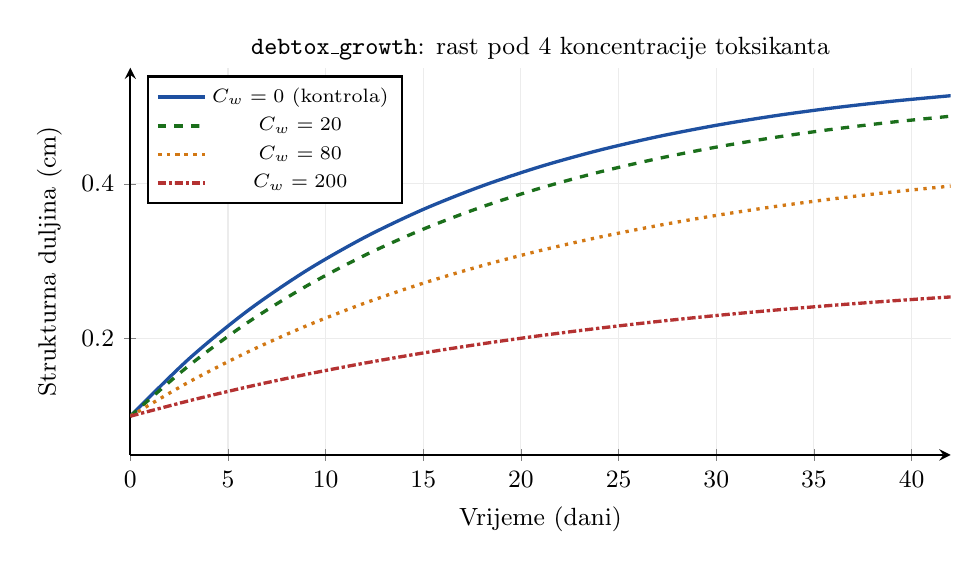
\begin{tikzpicture}
\begin{axis}[
    width=12cm, height=6.5cm,
    xlabel={Vrijeme (dani)},
    ylabel={Strukturna duljina (cm)},
    xmin=0, xmax=42, ymin=0.05, ymax=0.55,
    axis lines=left, thick,
    tick label style={font=\small},
    xlabel style={font=\small},
    ylabel style={font=\small},
    grid=major, grid style={gray!15},
    title={\small \code{debtox\_growth}: rast pod 4 koncentracije toksikanta},
    every axis title/.style={at={(0.5,1.05)}, font=\small},
    legend style={font=\scriptsize, at={(0.02,0.98)}, anchor=north west},
]
% Kontrola (C=0)
\addplot[debblue, very thick, smooth, domain=0:42, samples=15]
  {0.45 * (1 - exp(-0.06*x)) + 0.10};
\addlegendentry{$C_w = 0$ (kontrola)}

% C=20
\addplot[debgreen!80!black, very thick, smooth, dashed, domain=0:42, samples=15]
  {0.43 * (1 - exp(-0.055*x)) + 0.10};
\addlegendentry{$C_w = 20$}

% C=80
\addplot[deborange, very thick, smooth, dotted, domain=0:42, samples=15]
  {0.35 * (1 - exp(-0.045*x)) + 0.10};
\addlegendentry{$C_w = 80$}

% C=200
\addplot[debreduce, very thick, smooth, densely dashdotted,
         domain=0:42, samples=15]
  {0.20 * (1 - exp(-0.035*x)) + 0.10};
\addlegendentry{$C_w = 200$}

% Oznaka inhibicije
\draw[{Stealth[length=2mm]}-{Stealth[length=2mm]}, thick, debgrey]
  (43, 0.16) -- (43, 0.44);
\node[font=\scriptsize, text=debgrey, rotate=90] at (45, 0.30)
  {inhibicija rasta};
\end{axis}
\end{tikzpicture}
\caption{Ilustracija podataka \code{debtox\_growth}: srednje krivulje
  rasta pod četiri koncentracije toksikanta.  Veća koncentracija uzrokuje
  veću inhibiciju rasta putem smanjene asimilacije.}
\label{fig:debtox-podaci}
\end{figure}


% ============================================================
\section{Cjeloviti primjeri: Radni tokovi za sve tipove modela}
\label{sec:primjeri}


% ---- Primjer 1 ----
\begin{figure}[H]
\centering
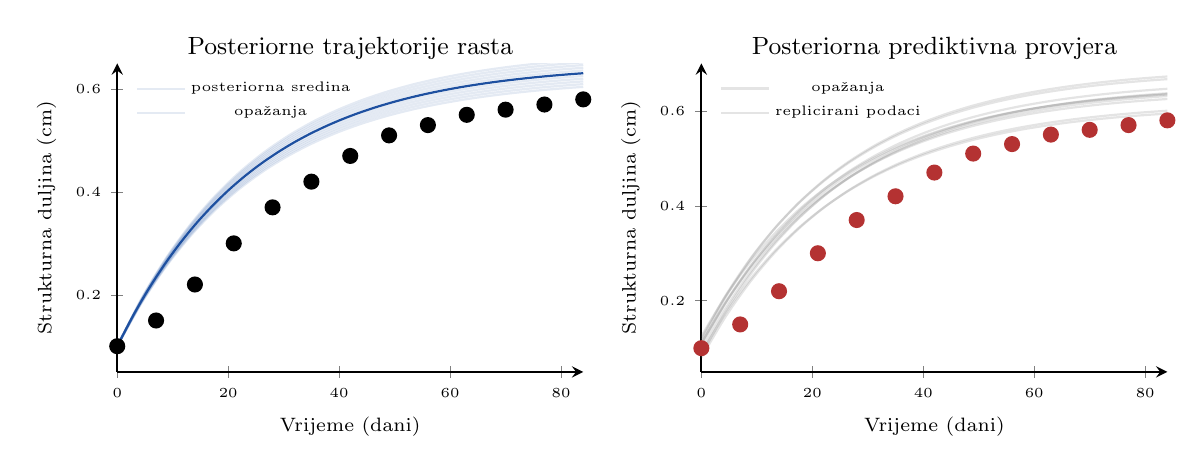
\begin{tikzpicture}
% --- Trajektorija rasta ---
\begin{axis}[
    name=traj, width=7.5cm, height=5.5cm,
    title={\small Posteriorne trajektorije rasta},
    xlabel={Vrijeme (dani)}, ylabel={Strukturna duljina (cm)},
    xmin=0, xmax=84, ymin=0.05, ymax=0.65,
    axis lines=left, thick,
    tick label style={font=\tiny},
    xlabel style={font=\scriptsize},
    ylabel style={font=\scriptsize},
    every axis title/.style={at={(0.5,1.05)}, font=\small},
    legend style={font=\tiny, at={(0.02,0.98)}, anchor=north west,
                  draw=none, fill=none},
]
% Posteriorne trajektorije (plave, prozirne)
\foreach \s in {0.98, 1.02, 0.95, 1.05, 0.97, 1.03, 0.99, 1.01, 0.96, 1.04} {
  \addplot[debblue, opacity=0.12, thick, smooth, domain=0:84, samples=20]
    {\s * 0.55 * (1 - exp(-0.04*x)) + 0.1};
}
% Srednja trajektorija
\addplot[debblue, thick, smooth, domain=0:84, samples=30]
  {0.55 * (1 - exp(-0.04*x)) + 0.1};
\addlegendentry{posteriorna sredina}

% Opazeni podaci (tocke)
\addplot[only marks, mark=*, mark size=2.5pt, black]
  coordinates {
    (0,0.10) (7,0.15) (14,0.22) (21,0.30) (28,0.37) (35,0.42)
    (42,0.47) (49,0.51) (56,0.53) (63,0.55) (70,0.56) (77,0.57) (84,0.58)
  };
\addlegendentry{opa\v{z}anja}
\end{axis}

% --- PPC: replicirani vs opazeni ---
\begin{axis}[
    at={(traj.east)}, anchor=west, xshift=15mm,
    width=7.5cm, height=5.5cm,
    title={\small Posteriorna prediktivna provjera},
    xlabel={Vrijeme (dani)}, ylabel={Strukturna duljina (cm)},
    xmin=0, xmax=84, ymin=0.05, ymax=0.70,
    axis lines=left, thick,
    tick label style={font=\tiny},
    xlabel style={font=\scriptsize},
    ylabel style={font=\scriptsize},
    every axis title/.style={at={(0.5,1.05)}, font=\small},
    legend style={font=\tiny, at={(0.02,0.98)}, anchor=north west,
                  draw=none, fill=none},
]
% Replicirani podaci (sive linije)
\foreach \s/\n in {0.97/0.01, 1.03/0.02, 0.95/-0.01, 1.05/0.015,
                   0.98/-0.02, 1.02/0.005, 0.96/0.025, 1.04/-0.015,
                   0.99/0.01, 1.01/-0.005} {
  \addplot[debgrey, opacity=0.2, thick, smooth, domain=0:84, samples=20]
    {\s * 0.55 * (1 - exp(-0.04*x)) + 0.1 + \n};
}
% Opazeni podaci (crvene tocke)
\addplot[only marks, mark=*, mark size=2.5pt, debreduce]
  coordinates {
    (0,0.10) (7,0.15) (14,0.22) (21,0.30) (28,0.37) (35,0.42)
    (42,0.47) (49,0.51) (56,0.53) (63,0.55) (70,0.56) (77,0.57) (84,0.58)
  };
\addlegendentry{opa\v{z}anja}
\addplot[debgrey, opacity=0.5, thick, no markers] coordinates {(0,0)(1,0)};
\addlegendentry{replicirani podaci}
\end{axis}
\end{tikzpicture}
\caption{Lijevo: posteriorne trajektorije rasta (plave linije) s
  opaženim podacima (crne točke).  Desno: posteriorna prediktivna
  provjera --- replicirani podaci (sive linije) trebaju obuhvatiti
  opažanja (crvene točke).}
\label{fig:trajektorija-ppc}
\end{figure}


\subsection{Primjer 1: Individualni model rasta}
\label{sec:primjer-individual}

Ovaj primjer pokazuje kompletni radni tok za procjenu DEB parametara
jedne jedinke gliste \textit{Eisenia fetida}.

\begin{lstlisting}
library(BayesianDEB)

# ============================================
# Korak 1: Priprema podataka
# ============================================
data(eisenia_growth)

# Odabir jedne jedinke
df1 <- eisenia_growth[eisenia_growth$id == 1, ]
dat <- bdeb_data(growth = df1, f_food = 1.0)
dat

# ============================================
# Korak 2: Specifikacija modela
# ============================================
mod <- bdeb_model(dat, type = "individual",
  priors = list(
    p_Am    = prior_lognormal(mu = 1.5, sigma = 0.5),
    p_M     = prior_lognormal(mu = -1.0, sigma = 0.5),
    kappa   = prior_beta(a = 3, b = 2),
    sigma_L = prior_halfnormal(sigma = 0.05)
  ))
mod  # ispisuje specifikaciju ukljucujuci sve priore

# ============================================
# Korak 3: Procjena putem MCMC
# ============================================
fit <- bdeb_fit(mod, chains = 4, iter_sampling = 2000,
                adapt_delta = 0.9, seed = 42)
fit  # ispisuje brzu dijagnosticku sumarizaciju

# ============================================
# Korak 4: Dijagnostika konvergencije
# ============================================
bdeb_diagnose(fit)
# Provjeriti:
#   - Nema divergentnih prijelaza
#   - Svi R-hat < 1.01
#   - Bulk ESS > 400 za sve parametre

# Trace grafovi
plot(fit, type = "trace")

# Posteriorne korelacije
plot(fit, type = "pairs",
     pars = c("p_Am", "p_M", "kappa"))

# ============================================
# Korak 5: Posteriorna sumarizacija
# ============================================
bdeb_summary(fit, prob = 0.95)

# ============================================
# Korak 6: Izvedene velicine
# ============================================
bdeb_derived(fit, quantities = c("L_inf", "growth_rate"))

# ============================================
# Korak 7: Posteriorna prediktivna provjera
# ============================================
ppc <- bdeb_ppc(fit, type = "growth")
plot(ppc, n_draws = 100)

# ============================================
# Korak 8: Grafikon trajektorija
# ============================================
plot(fit, type = "trajectory", n_draws = 200)
\end{lstlisting}


% ---- Primjer 2 ----
\subsection{Primjer 2: Hijerarhijski model s više jedinki}
\label{sec:primjer-hijerarhijski}

Hijerarhijski model koristi se kada imamo podatke za više jedinki i
želimo procijeniti populacijske distribucije parametara uz djelomično
spajanje (eng.\ partial pooling).  Model koristi necentriranu
parametrizaciju za individualne varijacije u $\{p_{Am}\}$.

\begin{figure}[H]
\centering
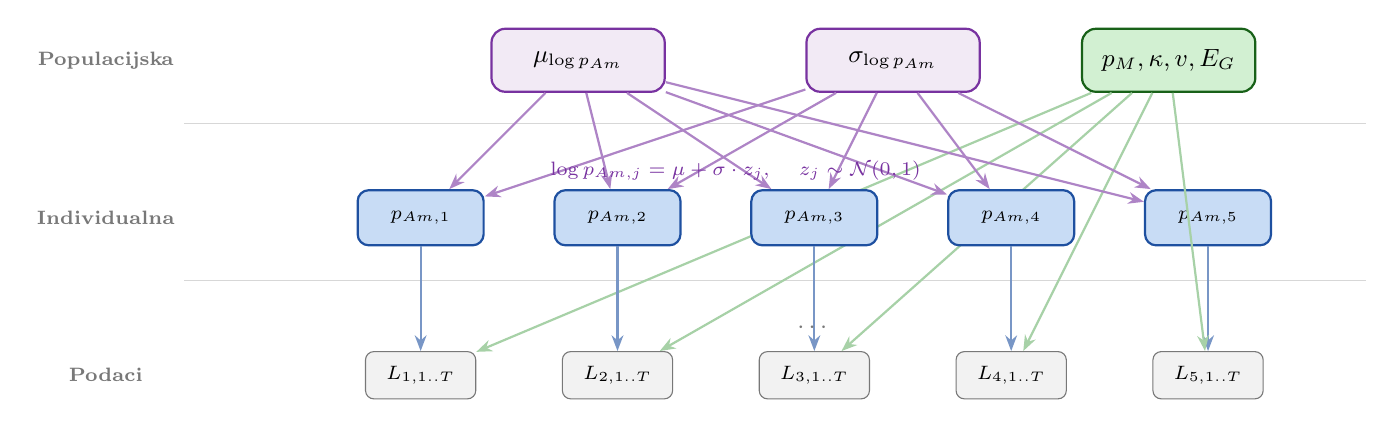
\begin{tikzpicture}[
    hyper/.style={rectangle, draw=debpurple, fill=debpurple!10,
                  rounded corners=5pt, thick, minimum width=2.2cm,
                  minimum height=0.8cm, font=\small},
    param/.style={rectangle, draw=debblue, fill=deblightblue,
                  rounded corners=4pt, thick, minimum width=1.6cm,
                  minimum height=0.7cm, font=\scriptsize},
    data/.style={rectangle, draw=debgrey, fill=gray!10,
                 rounded corners=3pt, minimum width=1.4cm,
                 minimum height=0.6cm, font=\scriptsize},
    arr/.style={-{Stealth[length=2mm]}, thick},
    level/.style={font=\scriptsize\bfseries, text=debgrey},
  ]
  % Razine
  \node[level] at (-3, 2.5) {Populacijska};
  \node[level] at (-3, 0.5) {Individualna};
  \node[level] at (-3, -1.5) {Podaci};

  % Horizontalne linije
  \draw[debgrey!30, thin] (-2, 1.7) -- (13, 1.7);
  \draw[debgrey!30, thin] (-2, -0.3) -- (13, -0.3);

  % Hiperparametri
  \node[hyper] (mu) at (3, 2.5)
    {$\mu_{\log p_{Am}}$};
  \node[hyper] (sigma) at (7, 2.5)
    {$\sigma_{\log p_{Am}}$};

  % Dijeljeni parametri
  \node[hyper, draw=debgreen!70!black, fill=deblightgreen]
    (shared) at (10.5, 2.5) {$p_M, \kappa, v, E_G$};

  % Individualni parametri
  \foreach \i/\x in {1/1, 2/3.5, 3/6, 4/8.5, 5/11} {
    \node[param] (p\i) at (\x, 0.5) {$p_{Am,\i}$};
    \draw[arr, debpurple!60] (mu) -- (p\i);
    \draw[arr, debpurple!60] (sigma) -- (p\i);
    % Podaci
    \node[data] (d\i) at (\x, -1.5) {$L_{\i,1..T}$};
    \draw[arr, debblue!60] (p\i) -- (d\i);
    \draw[arr, debgreen!40] (shared) -- (d\i);
  }

  % Oznaka necentrirane parametrizacije
  \node[font=\scriptsize, text=debpurple, align=center] at (5, 1.1)
    {$\log p_{Am,j} = \mu + \sigma \cdot z_j$, \quad $z_j \sim \mathcal{N}(0,1)$};

  % Tocke za vise jedinki
  \node[font=\small, text=debgrey] at (6, -0.9) {$\cdots$};
\end{tikzpicture}
\caption{Struktura hijerarhijskog modela.  Populacijski hiperparametri
  ($\mu_{\log p_{Am}}$, $\sigma_{\log p_{Am}}$) generiraju individualne
  stope asimilacije putem necentrirane parametrizacije.  Dijeljeni
  parametri ($p_M$, $\kappa$, $v$, $E_G$) utječu na sve jedinke
  jednako.}
\label{fig:hijerarhijski-struktura}
\end{figure}

\begin{lstlisting}
library(BayesianDEB)
data(eisenia_growth)

# ============================================
# Korak 1: Priprema (svih 21 jedinka)
# ============================================
dat_all <- bdeb_data(growth = eisenia_growth, f_food = 1.0)
dat_all
# => 21 jedinka, 273 opazanja

# ============================================
# Korak 2: Specifikacija hijerarhijskog modela
# ============================================
# Necentrirana parametrizacija automatski je
# implementirana u Stan modelu
mod_h <- bdeb_model(dat_all, type = "hierarchical",
  priors = list(
    mu_log_p_Am    = prior_normal(mu = 1.5, sigma = 0.5),
    sigma_log_p_Am = prior_exponential(rate = 2),
    kappa          = prior_beta(a = 3, b = 2)
  ))
mod_h

# ============================================
# Korak 3: Procjena (veci adapt_delta za slozeni model)
# ============================================
fit_h <- bdeb_fit(mod_h, chains = 4, iter_sampling = 2000,
                  adapt_delta = 0.95, seed = 123)

# ============================================
# Korak 4: Dijagnostika
# ============================================
bdeb_diagnose(fit_h)

# ============================================
# Korak 5: Populacijska sumarizacija
# ============================================
bdeb_summary(fit_h,
  pars = c("mu_log_p_Am", "sigma_log_p_Am",
           "p_M", "kappa", "v", "E_G"))

# ============================================
# Korak 6: Individualne stope asimilacije
# ============================================
bdeb_summary(fit_h,
  pars = paste0("p_Am_ind[", 1:21, "]"))

# ============================================
# Korak 7: Predikcija za novu (neopazenu) jedinku
# ============================================
# Stan model automatski generira p_Am_new u
# bloku generated quantities
bdeb_summary(fit_h, pars = "p_Am_new")

# ============================================
# Korak 8: Trace grafovi hijerarhijskih parametara
# ============================================
plot(fit_h, type = "trace",
  pars = c("mu_log_p_Am", "sigma_log_p_Am"))

plot(fit_h, type = "posterior",
  pars = c("mu_log_p_Am", "sigma_log_p_Am",
           "p_M", "kappa"))
\end{lstlisting}


% ---- Primjer 3 ----
\subsection{Primjer 3: Model rasta i reprodukcije}
\label{sec:primjer-repro}

Trodimenzionalni DEB model ($E$, $V$, $R$) procjenjuje istodobno
parametre rasta i reprodukcije.  Reproduktivni podaci modeliraju se
negativnom binomnom distribucijom za intervalske brojeve potomaka.

\begin{lstlisting}
library(BayesianDEB)

# ============================================
# Korak 1: Priprema podataka
# ============================================
growth_df <- data.frame(
  id = 1, time = seq(0, 56, by = 7),
  length = c(0.10, 0.18, 0.28, 0.37, 0.44,
             0.49, 0.52, 0.54, 0.55)
)

repro_df <- data.frame(
  id      = 1,
  t_start = c(28, 35, 42, 49),
  t_end   = c(35, 42, 49, 56),
  count   = c(5, 12, 18, 15)
)

dat_gr <- bdeb_data(growth = growth_df,
                    reproduction = repro_df,
                    f_food = 1.0)
dat_gr

# ============================================
# Korak 2: Specifikacija modela
# ============================================
mod_gr <- bdeb_model(dat_gr, type = "growth_repro",
  priors = list(
    kappa = prior_beta(a = 3, b = 2),
    k_R   = prior_lognormal(mu = -2, sigma = 1),
    E_Hp  = prior_lognormal(mu = 2.0, sigma = 1.5)
  ))

# ============================================
# Korak 3: Procjena
# ============================================
fit_gr <- bdeb_fit(mod_gr, chains = 4,
                   adapt_delta = 0.95, seed = 99)

# ============================================
# Korak 4: Dijagnostika i sumarizacija
# ============================================
bdeb_diagnose(fit_gr)
bdeb_summary(fit_gr)

# ============================================
# Korak 5: PPC za rast
# ============================================
plot(bdeb_ppc(fit_gr, type = "growth"))

# ============================================
# Korak 6: PPC za reprodukciju
# ============================================
plot(bdeb_ppc(fit_gr, type = "reproduction"))
\end{lstlisting}

\paragraph{Korištenje kumulativnih podataka.}
Ako su podaci o reprodukciji u kumulativnom obliku, prvo ih pretvorite:
\begin{lstlisting}
cumul <- data.frame(
  id         = rep(1, 6),
  time       = c(0, 14, 21, 28, 35, 42),
  cumulative = c(0, 0, 8, 25, 48, 72)
)
intervals <- repro_to_intervals(cumul)
dat_gr2 <- bdeb_data(growth = growth_df,
                     reproduction = intervals)
\end{lstlisting}


% ---- Primjer 4 ----
\subsection{Primjer 4: DEBtox ekotoksikološki model}
\label{sec:primjer-debtox}

Četverodimenzionalni TKTD model ($E$, $V$, $R$, $D_w$) procjenjuje
parametre DEB energetike i toksikološke parametre istodobno.  Ovaj
primjer koristi ugrađeni \code{debtox\_growth} dataset.

\begin{lstlisting}
library(BayesianDEB)

# ============================================
# Korak 1: Priprema podataka
# ============================================
data(debtox_growth)

# Mapiranje koncentracija
conc_map <- setNames(
  c(0, 20, 80, 200),
  as.character(unique(debtox_growth$concentration))
)

dat_tox <- bdeb_data(
  growth = debtox_growth,
  concentration = conc_map,
  f_food = 1.0
)
dat_tox

# ============================================
# Korak 2: Specifikacija DEBtox modela
# ============================================
mod_tox <- bdeb_tox(dat_tox, stress = "assimilation",
  priors = list(
    z_w = prior_lognormal(mu = 2.5, sigma = 1.0),
    b_w = prior_lognormal(mu = -5.0, sigma = 2.0),
    k_d = prior_lognormal(mu = -1.0, sigma = 1.0)
  ))
mod_tox

# ============================================
# Korak 3: Procjena
# ============================================
fit_tox <- bdeb_fit(mod_tox, chains = 4,
                    adapt_delta = 0.95, seed = 77)

# ============================================
# Korak 4: Dijagnostika
# ============================================
bdeb_diagnose(fit_tox)

# ============================================
# Korak 5: EC50 i NEC s 95% intervalima
# ============================================
ec_result <- bdeb_ec50(fit_tox, prob = 0.95)
# -- DEBtox Effect Concentrations ---
#   parameter  mean median    sd lower upper
#       EC50  ...   ...    ...   ...   ...
#        NEC  ...   ...    ...   ...   ...

# Histogram posteriorne distribucije EC50
hist(ec_result$draws, breaks = 40,
     main = "Posteriorna distribucija EC50",
     xlab = "Koncentracija")

# ============================================
# Korak 6: Krivulja doza-odgovor
# ============================================
plot_dose_response(fit_tox, n_draws = 200)

# ============================================
# Korak 7: Sumarizacija toksikoloskih parametara
# ============================================
bdeb_summary(fit_tox,
  pars = c("p_Am", "p_M", "kappa",
           "k_d", "z_w", "b_w", "sigma_L"))

# ============================================
# Korak 8: Trace i posteriorne gustoce
# ============================================
plot(fit_tox, type = "trace",
     pars = c("k_d", "z_w", "b_w"))

plot(fit_tox, type = "posterior",
     pars = c("k_d", "z_w", "b_w"))
\end{lstlisting}


% ============================================================
\begin{figure}[H]
\centering
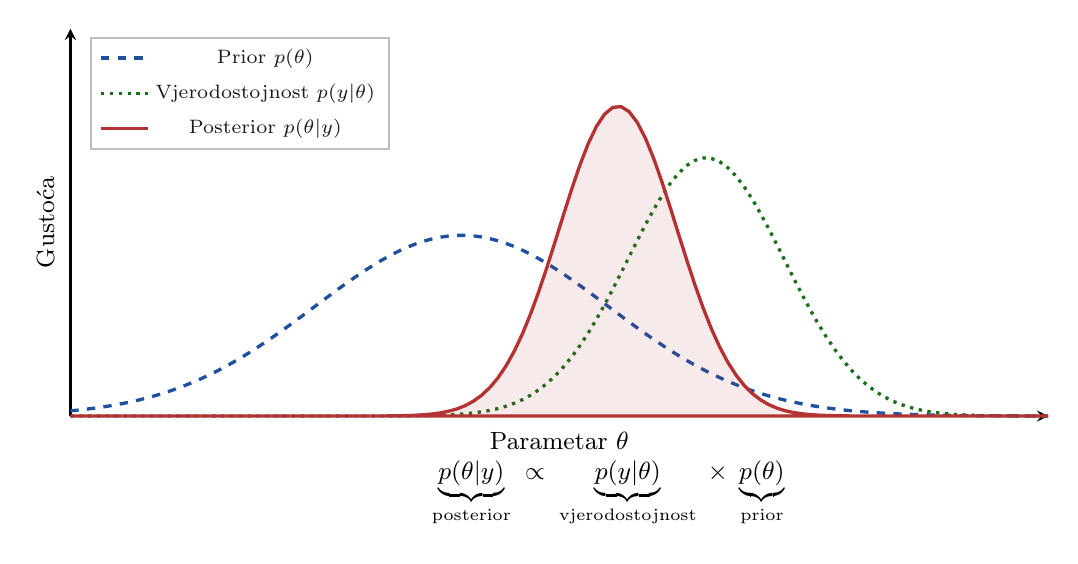
\begin{tikzpicture}
% --- Bayesovska inferencija: prior x likelihood = posterior ---
\begin{axis}[
    name=bayes, width=14cm, height=6.5cm,
    xlabel={Parametar $\theta$},
    ylabel={Gusto\'{c}a},
    xmin=-2, xmax=8, ymin=0, ymax=0.75,
    axis lines=left, thick,
    tick label style={font=\small},
    xlabel style={font=\small},
    ylabel style={font=\small},
    xtick=\empty, ytick=\empty,
    legend style={font=\scriptsize, at={(0.02,0.98)}, anchor=north west,
                  draw=gray!50, fill=white, fill opacity=0.9,
                  row sep=2pt},
    clip=false,
]
% Prior (siri, centriran na 2)
\addplot[debblue, very thick, dashed, domain=-2:8, samples=120]
  {0.35*exp(-(x-2)^2/(2*1.5^2))};
\addlegendentry{Prior $p(\theta)$}

% Likelihood (uzi, centriran na 4.5)
\addplot[debgreen!80!black, very thick, dotted, domain=-2:8, samples=120]
  {0.50*exp(-(x-4.5)^2/(2*0.8^2))};
\addlegendentry{Vjerodostojnost $p(y|\theta)$}

% Posterior (izmedu, centriran na ~3.6)
\addplot[debreduce, very thick, domain=-2:8, samples=120,
         fill=debreduce, fill opacity=0.1]
  {0.60*exp(-(x-3.6)^2/(2*0.6^2))} \closedcycle;
\addlegendentry{Posterior $p(\theta|y)$}

% Formula ispod grafa
\node[font=\small, align=center] at (3.5, -0.15)
  {$\underbrace{p(\theta|y)}_{\text{posterior}}
    \;\propto\; \underbrace{p(y|\theta)}_{\text{vjerodostojnost}}
    \;\times\; \underbrace{p(\theta)}_{\text{prior}}$};
\end{axis}
\end{tikzpicture}
\caption{Bayesovska inferencija: prior (isprekidana plava) kodira
  prethodno znanje, vjerodostojnost (točkasta zelena) sadrži informaciju
  iz podataka, a posterior (crvena) je rezultat njihovog kombiniranja
  putem Bayesovog teorema.  Posterior je uvijek uži od priora jer podaci
  pružaju dodatnu informaciju.}
\label{fig:bayesovska-inferencija}
\end{figure}


\section{Detalji Stan modela}
\label{sec:stan-detalji}

Ovaj odjeljak opisuje unutarnju strukturu ugrađenih Stan modela za
korisnike koji žele razumjeti ili proširiti ih.

\subsection{Desna strana DEB ODE sustava}

Svi modeli dijele istu ODE funkciju koja implementira jednadžbe
\eqref{eq:pA}--\eqref{eq:dV}.  Potpis funkcije u Stanu:

\begin{lstlisting}[style=Stanstyle]
vector deb_growth_ode(real t, vector x,
  array[] real theta, array[] real env)
\end{lstlisting}

gdje je \code{x = [E, V]'}, \code{theta = \{p\_Am, p\_M, kappa, v, E\_G\}},
i \code{env = \{f\}}.

Stabilizacijski član \code{1e-12} dodan je nazivniku mobilizacijskog
toka kako bi se spriječilo dijeljenje nulom:
\begin{equation}
\dot{p}_C = \frac{E\,v\,L}{E + [E_G]\,V + 10^{-12}}.
\end{equation}

\subsection{Hiperparametri priora kao podaci}

Hiperparametri priora prosljeđuju se iz \R-a kao Stan \code{data}
varijable (npr.\ \code{prior\_p\_Am\_mu}, \code{prior\_p\_Am\_sd}).  To
omogućuje korisnicima promjenu priora bez ponovnog kompiliranja Stan
modela.

\subsection{Necentrirana parametrizacija hijerarhijskog modela}

Hijerarhijski model koristi standardnu necentriranu parametrizaciju kako
bi izbjegao geometriju lijevka:
\begin{align}
  z_j &\sim \mathcal{N}(0, 1), \quad j = 1,\ldots,N, \\
  \log\{p_{Am}\}_j &= \mu_{\log p_{Am}} + \sigma_{\log p_{Am}} \cdot z_j.
\end{align}
Ovo razdvaja populacijske parametre ($\mu$, $\sigma$) od individualnih
devijacija i značajno poboljšava učinkovitost HMC uzorkovanja.

\begin{figure}[H]
\centering
\begin{tikzpicture}
% --- Centrirana (lijevak) ---
\begin{axis}[
    name=centred, width=7cm, height=6cm,
    title={\small Centrirana (lijevak)},
    xlabel={\scriptsize $\theta_j$},
    ylabel={\scriptsize $\sigma$},
    xmin=-4, xmax=4, ymin=0, ymax=3,
    axis lines=left, thick,
    tick label style={font=\tiny},
    xlabel style={font=\scriptsize},
    ylabel style={font=\scriptsize},
    every axis title/.style={at={(0.5,1.05)}, font=\small},
]
% Lijevak oblik - fiksne tocke
\addplot[only marks, mark=., mark size=1.5pt, debblue, opacity=0.5]
  coordinates {
    (0.01,0.1)(0.05,0.15)(-0.03,0.12)(0.08,0.2)(-0.06,0.18)
    (0.15,0.3)(-0.12,0.28)(0.2,0.4)(-0.18,0.35)(0.3,0.5)
    (-0.25,0.45)(0.4,0.6)(-0.35,0.55)(0.5,0.7)(-0.45,0.65)
    (0.6,0.8)(-0.55,0.75)(0.7,0.9)(-0.65,0.85)(0.8,1.0)
    (-0.75,0.95)(1.0,1.1)(-0.9,1.05)(1.1,1.2)(-1.0,1.15)
    (1.3,1.3)(-1.2,1.25)(1.4,1.4)(-1.3,1.35)(1.6,1.5)
    (-1.5,1.45)(1.7,1.6)(-1.6,1.55)(1.9,1.7)(-1.8,1.65)
    (2.0,1.8)(-1.9,1.75)(2.2,1.9)(-2.1,1.85)(2.3,2.0)
    (-2.2,1.95)(2.5,2.1)(-2.4,2.05)(2.6,2.2)(-2.5,2.15)
    (2.8,2.3)(-2.7,2.25)(2.9,2.4)(-2.8,2.35)(3.0,2.5)
    (-2.9,2.45)(3.1,2.6)(-3.0,2.55)(3.2,2.7)(-3.1,2.65)
    (0.1,0.25)(-0.08,0.22)(0.35,0.5)(-0.3,0.48)(0.9,0.95)
    (-0.85,0.92)(1.5,1.45)(-1.4,1.42)(2.1,1.92)(-2.0,1.88)
    (2.7,2.35)(-2.6,2.32)(1.8,1.68)(-1.7,1.62)(0.45,0.62)
    (-0.4,0.58)(1.2,1.22)(-1.1,1.18)(0.02,0.13)(-0.01,0.11)
  };
\draw[debreduce, thick, dashed] (-0.3, 0.05) -- (0.3, 0.05)
  -- (3, 2.8) -- (-3, 2.8) -- cycle;
\end{axis}

% --- Necentrirana (bolja geometrija) ---
\begin{axis}[
    at={(centred.east)}, anchor=west, xshift=15mm,
    width=7cm, height=6cm,
    title={\small Necentrirana},
    xlabel={\scriptsize $z_j$},
    ylabel={\scriptsize $\sigma$},
    xmin=-4, xmax=4, ymin=0, ymax=3,
    axis lines=left, thick,
    tick label style={font=\tiny},
    xlabel style={font=\scriptsize},
    ylabel style={font=\scriptsize},
    every axis title/.style={at={(0.5,1.05)}, font=\small},
]
% Ravnomjernije rasprsene tocke
\addplot[only marks, mark=., mark size=1.5pt, debgreen!80!black, opacity=0.5]
  coordinates {
    (-2.5,0.3)(1.8,0.5)(-0.5,0.8)(2.1,1.2)(-1.3,1.5)(0.8,0.4)
    (-2.0,1.8)(1.5,2.1)(-0.8,2.5)(2.5,0.7)(-1.8,1.1)(0.3,1.6)
    (-2.3,2.0)(1.2,2.4)(-0.2,0.2)(2.8,1.4)(-1.5,2.3)(0.6,0.9)
    (-2.7,1.3)(1.0,1.7)(0.1,2.2)(-1.0,0.6)(2.3,2.6)(-0.6,1.9)
    (1.7,0.3)(-2.1,2.8)(0.5,1.0)(-1.7,0.4)(2.0,1.8)(-0.3,2.7)
    (1.3,0.6)(-2.4,1.6)(0.9,2.3)(-1.2,0.8)(2.6,1.0)(-0.9,1.3)
    (1.6,2.0)(-2.6,0.5)(0.2,1.4)(-1.4,2.1)(2.2,0.9)(-0.4,0.3)
    (1.1,2.7)(-1.9,1.2)(0.7,0.1)(2.4,2.2)(-0.7,1.7)(1.4,1.1)
    (-2.2,2.5)(0.4,0.7)(-1.6,1.9)(1.9,1.5)(-0.1,2.4)(2.7,0.2)
    (-1.1,0.5)(0.0,1.8)(2.9,1.3)(-2.8,0.9)(1.1,2.1)(-0.5,1.1)
    (1.8,2.8)(-2.3,0.7)(0.6,1.5)(-1.3,2.6)(2.1,0.4)(-0.8,2.0)
    (1.5,0.8)(-2.5,1.4)(0.3,2.9)(-1.0,1.0)(2.4,1.7)(-0.2,0.6)
    (1.2,1.9)(-1.8,2.2)(0.8,0.5)(2.0,2.4)
  };
\end{axis}
\end{tikzpicture}
\caption{Usporedba geometrije posteriorne distribucije.  Lijevo:
  centrirana parametrizacija stvara geometriju lijevka koja otežava HMC
  uzorkovanje.  Desno: necentrirana parametrizacija daje ravnomjerniju
  geometriju.}
\label{fig:lijevak}
\end{figure}

\subsection{Generated quantities}

Svi Stan modeli u bloku \code{generated quantities} generiraju:
\begin{itemize}[nosep]
  \item \code{L\_rep} --- replicirane duljine za posteriorne prediktivne provjere,
  \item \code{log\_lik} --- log-vjerodostojnost po opažanju (za usporedbu modela putem LOO-CV),
  \item \code{EC50}, \code{NEC} --- samo za DEBtox model,
  \item \code{p\_Am\_new} --- samo za hijerarhijski model (predikcija za novu jedinku).
\end{itemize}


% ============================================================
\section{Praktični savjeti}
\label{sec:savjeti}

\subsection{Odabir \code{adapt\_delta}}

Počnite s \code{adapt\_delta = 0.8} (zadano).  Ako \fn{bdeb\_diagnose}
prijavi divergentne prijelaze, povećajte na 0.9, 0.95 ili čak 0.99.
Više vrijednosti usporavaju uzorkovanje, ali poboljšavaju geometrijsku
vjernost.

\begin{lstlisting}
# Pocetni pokusaj
fit <- bdeb_fit(mod, adapt_delta = 0.8)
bdeb_diagnose(fit)  # ako ima divergencija:

# Povecani adapt_delta
fit <- bdeb_fit(mod, adapt_delta = 0.95)
\end{lstlisting}

\subsection{Kada koristiti hijerarhijski model}

Koristite \code{type = "hierarchical"} kada:
\begin{itemize}[nosep]
  \item Imate podatke za više od 3--4 jedinke.
  \item Želite procijeniti populacijske distribucije parametara.
  \item Neke jedinke imaju rijetke podatke (djelomično spajanje pomaže).
  \item Trebate predikcije za nove, neopažene jedinke.
\end{itemize}

\subsection{Osjetljivost na priore}

Uvijek usporedite rezultate pod barem dvije vjerodostojne specifikacije
priora.  Parametri koji ostaju dominirani priorom (posteriorna
distribucija $\approx$ priorna distribucija) slabo su identificirani i
trebaju se tako prijaviti.

\begin{lstlisting}
# Specifikacija 1: siri priori
mod1 <- bdeb_model(dat, type = "individual",
  priors = list(
    p_Am = prior_lognormal(mu = 1.5, sigma = 1.0)
  ))

# Specifikacija 2: uzi priori
mod2 <- bdeb_model(dat, type = "individual",
  priors = list(
    p_Am = prior_lognormal(mu = 1.5, sigma = 0.3)
  ))

fit1 <- bdeb_fit(mod1, seed = 42)
fit2 <- bdeb_fit(mod2, seed = 42)

# Usporedba posteriornih sumarizacija
bdeb_summary(fit1, pars = "p_Am")
bdeb_summary(fit2, pars = "p_Am")
\end{lstlisting}

\subsection{Računalni savjeti}

\begin{itemize}[nosep]
  \item Kompilacija Stan modela je spora prvi put ($\sim$30\,s), ali se
    kešira za buduće procjene.
  \item Koristite \code{parallel\_chains = 4} za paralelno pokretanje
    lanaca.
  \item Za velike hijerarhijske modele, počnite s podskupom jedinki za
    testiranje parametrizacije, zatim proširite.
  \item Ako ODE rješavač zakaže, provjerite početne uvjete (\code{E0},
    \code{L0}) i osigurajte da su biološki razumne.
  \item Za tihi rad koristite \code{refresh = 0}.
\end{itemize}


% ============================================================
\section{Usporedba s postojećim alatima}
\label{sec:usporedba}

\begin{table}[htbp]
\centering
\caption{Usporedba paketa \pkg{BayesianDEB} s postojećim alatima za DEB kalibraciju.}
\label{tab:usporedba}
\begin{tabular}{lcccc}
\toprule
\textbf{Značajka} & \textbf{AmP/DEBtool} & \textbf{deBInfer} & \textbf{Ručni Stan} & \textbf{BayesianDEB} \\
\midrule
Bayesovska inferencija      & --          & Da  & Da  & Da \\
Ugrađeni DEB modeli         & Da          & --  & --  & Da \\
Hijerarhijski modeli        & --          & --  & Ručno & Ugrađeno \\
DEBtox (TKTD)               & Djelomično  & --  & Ručno & Ugrađeno \\
API za priore               & --          & Osnovni & Ručno & Bogat \\
Dijagnostika                & Minimalna   & Osnovna & Ručno & Automatska \\
PPC                         & --          & --  & Ručno & Ugrađeno \\
\R{} paket                  & MATLAB+\R{} & Da  & --  & Da \\
\bottomrule
\end{tabular}
\end{table}


% ============================================================
\section{Pregled svih eksportiranih funkcija}
\label{sec:pregled-funkcija}

\begin{longtable}{lll}
\toprule
\textbf{Funkcija} & \textbf{Kategorija} & \textbf{Opis} \\
\midrule
\endhead
\fn{bdeb\_data} & Priprema & Validira i strukturira ulazne podatke \\
\fn{repro\_to\_intervals} & Priprema & Pretvara kumulativnu u intervalsku reprodukciju \\
\midrule
\fn{prior\_lognormal} & Priori & Log-normalna priorna distribucija \\
\fn{prior\_normal} & Priori & Normalna priorna distribucija \\
\fn{prior\_beta} & Priori & Beta priorna distribucija \\
\fn{prior\_halfnormal} & Priori & Polu-normalna priorna distribucija \\
\fn{prior\_halfcauchy} & Priori & Polu-Cauchyjeva priorna distribucija \\
\fn{prior\_exponential} & Priori & Eksponencijalna priorna distribucija \\
\fn{prior\_default} & Priori & Zadani slabo informativni priori \\
\midrule
\fn{obs\_normal} & Opažanja & Gaussovska pogreška \\
\fn{obs\_lognormal} & Opažanja & Log-normalna pogreška \\
\fn{obs\_student\_t} & Opažanja & Studentova t pogreška \\
\fn{obs\_poisson} & Opažanja & Poissonova distribucija \\
\fn{obs\_negbinom} & Opažanja & Negativna binomna distribucija \\
\midrule
\fn{bdeb\_model} & Specifikacija & Kombinira podatke, tip, priore, opažanja \\
\fn{bdeb\_tox} & Specifikacija & Pogodnosna ovojnica za DEBtox \\
\midrule
\fn{bdeb\_fit} & Procjena & MCMC uzorkovanje putem cmdstanr-a \\
\midrule
\fn{bdeb\_diagnose} & Dijagnostika & Konvergencija, R-hat, ESS, E-BFMI \\
\fn{bdeb\_summary} & Dijagnostika & Posteriorna sumarizacija parametara \\
\fn{bdeb\_derived} & Dijagnostika & Izvedene biološke veličine \\
\midrule
\fn{bdeb\_ppc} & PPC & Posteriorne prediktivne provjere \\
\fn{bdeb\_predict} & Predikcija & Posteriorne prediktivne trajektorije \\
\midrule
\fn{bdeb\_ec50} & DEBtox & Ekstrakcija EC50 i NEC \\
\fn{plot\_dose\_response} & DEBtox & Krivulja doza-odgovor \\
\midrule
\fn{arrhenius} & Pomoćne & Arrheniusova temperaturna korekcija \\
\fn{deb\_fluxes} & Pomoćne & Izračun DEB energetskih tokova \\
\midrule
\code{plot.bdeb\_fit} & S3 metoda & Trace, posterior, pairs, trajectory \\
\code{plot.bdeb\_ppc} & S3 metoda & Vizualizacija PPC-a \\
\code{print.bdeb\_data} & S3 metoda & Ispis sumarizacije podataka \\
\code{print.bdeb\_model} & S3 metoda & Ispis specifikacije modela \\
\code{print.bdeb\_fit} & S3 metoda & Ispis rezultata procjene \\
\code{print.bdeb\_ppc} & S3 metoda & Ispis PPC sumarizacije \\
\code{summary.bdeb\_fit} & S3 metoda & Poziva \fn{bdeb\_summary} \\
\code{predict.bdeb\_fit} & S3 metoda & Poziva \fn{bdeb\_predict} \\
\bottomrule
\end{longtable}


% ============================================================
\section*{Literatura}

\begin{itemize}[nosep]
  \item Kooijman, S.A.L.M.\ (2010).\ \textit{Dynamic Energy Budget Theory
    for Metabolic Organisation}.  Cambridge University Press.
    \texttt{doi:10.1017/CBO9780511805400}
  \item Carpenter, B.\ et al.\ (2017).\ Stan: A Probabilistic Programming
    Language.\ \textit{Journal of Statistical Software}, 76(1).
  \item Gelman, A.\ et al.\ (2020).\ \textit{Bayesian Data Analysis},
    3rd ed.\ Chapman \& Hall/CRC.
  \item Jager, T.\ \& Zimmer, E.I.\ (2012).\ Simplified Dynamic Energy
    Budget model for analysing ecotoxicity data.\ \textit{Ecological
    Modelling}, 225, 74--81.
\end{itemize}

\end{document}
